\documentclass[article, onecolumn, draftclsnofoot,10pt, compsoc]{IEEEtran}
\usepackage{graphicx}
\usepackage{url}
\usepackage{setspace}
\usepackage[usenames,dvipsnames,svgnames,table]{xcolor}
%\usepackage{lipsum}
\usepackage{csquotes}
\usepackage[parfill]{parskip}
\usepackage{pgfgantt}
\parindent=0pt
\usepackage{geometry}
\usepackage{float}
\geometry{textheight=9.5in, textwidth=7in}

% 1. Fill in these details
\def \CapstoneTeamName{		SigFind}
\def \CapstoneTeamNumber{		65}
\def \GroupMemberOne{			Jacob Geddings}
\def \GroupMemberTwo{			Inhyuk Lee}
\def \GroupMemberThree{			Juan Mugica}
\def \CapstoneProjectName{		CDK Data Stream AI}
\def \CapstoneSponsorCompany{	CDK Global}
\def \CapstoneSponsorPerson{		Chris Smith}

% 2. Uncomment the appropriate line below so that the document type works
\def \DocType{		%Problem Statement
				%Requirements Document
				%Technology Review
				%Design Document
				Final Progress Report
				}
			
\newcommand{\NameSigPair}[1]{\par
\makebox[2.75in][r]{\backslash 1} \hfil 	\makebox[3.25in]{\makebox[2.25in]{\hrulefill} \hfill		\makebox[.75in]{\hrulefill}}
\par\vspace{-12pt} \textit{\tiny\noindent
\makebox[2.75in]{} \hfil		\makebox[3.25in]{\makebox[2.25in][r]{Signature} \hfill	\makebox[.75in][r]{Date}}}}
% 3. If the document is not to be signed, uncomment the RENEWcommand below
%\renewcommand{\NameSigPair}[1]{\backslash 1}

%%%%%%%%%%%%%%%%%%%%%%%%%%%%%%%%%%%%%%%
\begin{document}
\begin{titlepage}
    \pagenumbering{gobble}
    \begin{singlespace}
    	\includegraphics[height=4cm]{coe_v_spot1}
        \hfill 
        % 4. If you have a logo, use this includegraphics command to put it on the coversheet.
        %\includegraphics[height=4cm]{CompanyLogo}   
        \par\vspace{.2in}
        \centering
        \scshape{
            \huge CS Capstone \DocType \par
            {\large\today}\par
            \vspace{.5in}
            \textbf{\Huge\CapstoneProjectName}\par
            \vfill
            {\large Prepared for}\par
            \Huge \CapstoneSponsorCompany\par
            \vspace{5pt}
            {\Large\CapstoneSponsorPerson\par}
            {\large Prepared by }\par
            Group\CapstoneTeamNumber\par
            % 5. comment out the line below this one if you do not wish to name your team
            \CapstoneTeamName\par 
            \vspace{5pt}
            {\Large
                \GroupMemberOne\par
                \GroupMemberTwo\par
               \GroupMemberThree\par
            }
            \vspace{20pt}
        }
        \begin{abstract}
        % 6. Fill in your abstract    
		
        \end{abstract}     
    \end{singlespace}
\end{titlepage}
\newpage
\pagenumbering{arabic}
\tableofcontents
% 7. uncomment this (if applicable). Consider adding a page break.
%\listoffigures
%\listoftables
\clearpage

% 8. now you write!
% \\\\\\\\\\\\\\\\\\\\\\\Introduction to Project\\\\\\\\\\\\\\\\\\\\\\\
\section{Introduction to Project}
\subsection{Who is our client}
CDK Global currently operates with thousands of different dealerships across the world each of which using their own unique forms, servers, and verification methods for each transaction. The company is interested in providing new forward-thinking solutions to the various logistical problems that surface as a result of permitting such liberties within their various branches. Our direct correspondent and client from CDK Global is Chris Smith, who went on to provide an advisory role for the project as it progressed through the development lifecycle.

\subsection{Defininf the problem}
As mentioned, the current system has allowed a great level of liberty for each dealership but has made it a logistical nightmare to quickly coordinate documents and to ensure everything submitted is actually valid. In particular, their main concern is finding a way to quickly verify if a form has been signed. Beyond that core issue they are also interested in reigning in their various servers so that this verification process is done under one roof and with a singular database. To achieve this task, CDK Global does have a few ground rules regarding the development of any potential solutions. They are interested in an open-source design with no licensing requirements and to have it modular in nature to ensure upgrades can be carried out as needed should our solution be implemented.

\subsection{Why this is important}
The current model being used to tackle this problem is to have dedicated employees devote their entire workday to the manual scanning and verification of documents. This process is not only sluggish in nature but very accident prone with an extreme dependency on human error not occurring. Not only that but this occurs only after the fact when considering potential transactions. A worst-case scenario could be an auto dealership releasing a car to a potential buyer to only realize there was no legally binding signature proving the purchase of the vehicle. By implementing AI assistance, we can permit quick feedback on submitted documents as well as significantly reduce the cost to the company in verification by mitigating errors and reducing manpower necessary to being devoted to this fact-checking process.

\subsection{Our team}
Our team, Group 65, was created to tackle this problem. Within our team is three members: Jacob Geddings, Inhyuk Lee, and Juan Mugica. This team was assembled based on the common interest of wanting to explore what goes into AI development and found this project to be a perfect opportunity to work with these new concepts. While we ultimately named our project ‘SigFind’ we also would use the term to refer to our group instead of the generic number classification. Overall, our group was expected to spend the Fall term working on research and documentation for the project with Winter representing the coding phase and Spring acting as our debugging and finalization of the project for code handoff.

Jacob Geddings would function as team leader for the duration of this project. Most notable contributions can be found in documentation, client communication, and organization of the project. This meant that Fall and Spring was particularly workload heavy for Geddings whereas Winter was a comparatively lighter workload for dedicated tasks. During the coding phase of Winter term, he contributed towards our file conversion module as his dedicated portion of the project. Given that the file conversion was a quick implementation he would spend the remainder of coding working on providing assistance with OCR Tesseract as well as constructing training sets for our Convolutional Network. 

Inhyuk Lee functioned as second in command for the team and, when able, provided a second set of notes on most interactions within the group and with our client. His primary task was to develop the OCR Tesseract component of our project. This meant creating a program that could correctly analyze any arbitrary page and locate potential signature lines. Once that could be detected he was then tasked with cropping those signature lines out to submit to our convolutional network. Lastly, Lee also provided assistance in submitting samples for the training set of our program.

Juan Mugica was our dedicated convolutional network researcher and implementer. Due to the importance of this module it was deemed best to have at least one member be completely focused on this component and not be concerned with the other modules as much. During the Fall term, Juan explored potential AI platforms for our network. From then on his entire focus was towards the correct creation of the network and ensuring proper judgement capacity of the program when interpreting signature lines.

% \\\\\\\\\\\\\\\\\\\\\\\Requirmentrs Document\\\\\\\\\\\\\\\\\\\\\\\
\section{Requirmentrs Document}
\subsection{Introduction}
\subsubsection{Purpose}
The purpose of this requirements document is to bring clarity to the project by indicating what the hard-line requirements are for the project to be considered a success. This will be done with the consideration that the desired end product may not be achievable and as a result will be treated as a form of research project or proof of concept.

Intended target audience for this document is our client and by extension CDK[1] given this is their idea and the success of the project directly assists them. In addition, our instructors and teaching assistant are extensively involved in this project and they will be using this as a grading guideline. The assumption is that the reader is familiar with general concepts within computer science including artificial intelligence, common programming languages, and coding environments.


\subsubsection{Scope}
The product being developed will be a variant of open source AI that will be tailored to scanning submitted forms by CDK. With the inclusion of stretch goals this platform may also analyze driver licenses, vehicle imaging, or name to vehicle identification. 

This project will be capable of analyzing a submitted form to locate its signature box and check to see if it has been signed. It will also prompt the operator if it is not certain of what it is observing and if a cosigner box is also present. The format of these submissions will be in PDF format. Stretch goals include the capacity to detect expiration dates on driver’s licenses and determine what make and model of a vehicle is based on a submitted image. Additional file formats are also being considered.

Benefits from this product include reduced costs for CDK in error checking forms, rapid validation of a document, and a singular platform that can scan the various form styles that CDK possesses. Another goal of this design is the ability for it to expand upon itself and adapt to new forms that may be introduced by permitting operator confirmation or override on its assessment. 

\subsubsection{Definitions, Acronyms, and Abbreviations}
Open source AI is a free to access platform in which the code can be used and implemented as seen fit by the operator. OpenCV[2] is a popular image processing example of this as well as TensorFlow[3] and DL4j[4]. Programming languages that may be used include C++[5], Python[6], and Java[7]. The use of an IDE is likely, which means Integrated Development Environment which provides a more convenient setup for coding. Examples of IDE’s include Microsoft Visual Studio[8] and Eclipse[9]. Black box design means that the user does not need to understand the internal functions of the program, just what it wants as input and what the user will receive as the output. 

\subsubsection{References}
[1] "CDK Global" Internet: https://www.cdkglobal.com/, 2017 [Nov. 10, 2017].

[2] "OpenCV" Internet: https://opencv.org/, Aug. 3, 2017 [Nov. 11, 2017].

[3] "TensorFlow" Internet: https://www.tensorflow.org/, [Nov. 12, 2017].

[4] "Deeplearning4j" Internet: https://deeplearning4j.org/, 2017 [Nov. 11, 2017].

[5] "C++" Internet: http://www.cplusplus.com/, 2017 [Nov. 12, 2017].

[6] "Python" Internet: https://www.python.org/, Oct. 17, 2017 [Nov. 12, 2017].

[7] "Java" Internet: https://java.com/en/, Apr. 22, 2016 [Nov. 12, 2017].

[8] "Microsoft Visual Studio" Internet: https://www.visualstudio.com/, Oct. 2016 [Nov. 10, 2017].

[9] "Eclipse" Internet: https://www.eclipse.org/ide/, 2017 [Nov. 9, 2017].

[10] IEEE Software Engineering Standards Committee, “IEEE Std 830-1998, IEEE Recommended Practice for Software Requirements Specifications”, June 25, 1998.

[11] "GCC" Internet: https://gcc.gnu.org/, Nov. 3, 2017 [Nov. 9, 2017].

[12] "CMake" Internet: https://cmake.org/, Nov. 10, 2017 [Nov. 9, 2017].

\subsubsection{Overview}
The remainder of the requirements document will contain a greater look into what precisely the project entails. This is going to involve looking at where the project stands for CDK and how it will be utilized as well as the products functions and characteristics for a user. Mention will also be made towards potential constraints placed upon the program.

The following section will be a general overview and description of the project, primary focus being placed on functions, characteristics, constraints, and assumptions/dependencies. After that there will be a section on specific requirements that will bring mention to potential interfacing concerns as well as performance metrics and standards compliance. The document is designed to follow the IEEE Software Engineering Standards [10].


\subsection{Overall Description}
\subsubsection{Product Perspective}
The core objective as well as the stretch goals all conclude that this product will be an independent platform. For this project, we will explore the potential of A.I. and create the foundation of CDK’s own AI platform.

The signature detection and drivers license verification software must support various personal computers such as desktop, laptop, and tablet as an input source. This software will first receive a PDF file of a document as its input. It will then compute the data and give result or feedback to user. With that in mind, the software needs to be robust enough to compute large set of data. Similarly, within our stretch goals, vehicle model detection software must also support various personal computers and be robust enough to evaluate large data. However, it must also support portable devices with camera such as phone and tablet. Software should first take photo from camera then it evaluates the photo and returns model number.

\subsubsection{Product Functions}
Main goal
The function of this software is detecting the location of the signature box and determine whether it is signed or unsigned. If document is unsigned: software must provide information of location and quantity of missing components. Also, the program must be capable of making a reasonable guess on whether a signature is sufficiently binding. This entails the AI must be capable of distinguishing between a simple mark in the signature window and an actual signature.

Stretch goal
License validation software: This software must validate whether given photo is driver’s license or not. First, it must validate the format of driver’s license and check legal information such as expiration date.

Vehicle model detection software: Vehicle model detection software must be able to determine the specific model number from appearance of the vehicle. Software will first take photos or video of vehicle taken from different angle. It will determine vehicle model by narrowing down the information. For example, software will search sequentially for make, model, and year.

\subsubsection{User Characteristics}
The intended user of the software is vehicle retailers. We can assume a low degree of understanding on artificial intelligence. Therefore, software must be designed as black box model. To accompany this structure the user interface must be agreeable for them. Lastly, the program must not overburden the operator, it will take a single file as input to scan and return a conclusion to the user.


\subsubsection{Constraints}
There are few constraints on CDK A.I. data stream project. First, software must be standalone. The future goal of this project is to build CDK’s own platform, so software must be independent. In addition, project must be kept in open source. The software must be made in such a way that, once our team has completed its work, the project be taken over by a new team within CDK. To meet this demand the need for thorough documentation of implementation is vital. This project will also have limits on testing due to the privacy issue surrounding actual consumer data. Since the data that signature detecting and license validation software compute contains personal data, testing data must be done on dummy documents and licenses. The last constraint is that product must function on its own without the additional use or maintenance of outside software. Since the users of the product are unlikely to be familiar with the internal workings the interface for them must sufficiently mask the technical workings of the program only provide a clean and simple menu.

\subsubsection{Assumptions and Dependencies}

All images provided by the client are sanitized and free of legal conflicts. Cloud based deployment services will be provided by the client. From a developing and testing standpoint, this project will be developped in C++ utilizing the OpenCV picture formatting library. This library assumes that the system is running GCC 4.4.x[11] or later as well as CMake 2.8.7[12] or higher. 



\subsection{Specific Requirements}

\subsubsection{External Interface Requirements}
The focus of this project is building signature detecting artificial intelligence run on the CDK server. It must be designed as black box model, so user interface must be simple . Since software runs on the CDK server, communication interface must be secure and durable. 

The structure of user interface is very simple. There are two functions in user interface. Software simply takes set of documents from the user, and it displays result of the signature detection to the user. Result of the signature will be any pages of the document where error is detected.

Communication between our software and the CDK server database is important; however, focus on this project is making accurate and reliable artificial intelligence. We are considering the use of docker and amazon web services to construct a reliable communication structure but this is a stretch goal of the project.

\subsubsection{System Features}
\paragraph{Signature detecting capability}\vspace{.5cm}
\begin{description}
\item [] Introduction/Purpose of feature: The program must be able to detect if a document contains a signature regardless of the documents formatting.
\item [] Stimulus/Response sequence: The program will parse a PDF image of a document, or a document in PDF format, and output a percentage based estimation as to whether it contains a signature.
\item [] Functional Requirements: Signature detection must be functional for all types of document formats regardless of the type so long as they are presented in PDF file format. 
\end{description}



\paragraph{Missing signature detection}\vspace{.5cm}
\begin{description}
\item [] Introduction/Purpose of feature: The program must be able to detect if a document contains a space where there should be a signature regardless of the format of the form.
\item [] Stimulus/Response sequence: The program will parse a PDF image of a document , or a document in PDF format, and output a percentage based estimation as to whether it contains a space where a signature is missing.
\item [] Functional Requirements: Signature detection must be functional for all types of document formats regardless of the type so long as they are presented in PDF file format. 
\end{description}

\paragraph{Multiple signature and multiple missing signature capability}\vspace{.5cm}
\begin{description}
\item [] Introduction/Purpose of feature: The program must be able to perform feature 3.2.1 for every signature contained within the document. The program must also be able to perform feature 3.2.2 for every space that is missing a signature within the document.
\item [] Stimulus/Response sequence: The program will parse a PDF image of a document, or a document in PDF format, and output percent estimates for features 3.2.1 and 3.2.2 at every instance deemed applicable. 
\item [] Functional Requirements: Multiple signature and multiple missing signature capabilities must be functional for all types of document formats regardless of the type so long as they are presented in PDF file format.
\end{description}

\vspace{.75cm}
\textbf{\textit{The following features are part of the groups stretch goals and are to be completed once the aforementioned features work to the satisfaction of the client. 
}}
\vspace{.75cm}


\paragraph{Car detection within image}\vspace{.5cm}
\begin{description}
\item [] Introduction/Purpose of feature: The program must detect if a given picture contains a car within it.
\item [] Stimulus/Response sequence: The program will parse a PDF image and output a percentage based estimate as to whether it contains a car.
\item [] Functional Requirements: The program must be able to detect cars within any picture presented in PDF format.
\end{description}

\paragraph{License and Permit detection within document}\vspace{.5cm}
\begin{description}
\item [] Introduction/Purpose of feature: The program must detect if a document contains a license or a permit regardless of the format of the form.
\item [] Stimulus/Response sequence: The program will parse a PDF image of a document , or a document in PDF format, and output a percentage based estimation as to whether it contains a license, or a permit.
\item [] Functional Requirements: The program must be able to detect permits and licenses within any document presented in PDF format.
\end{description}

\paragraph{Parse license plate, license, and permit text into machine readable format}\vspace{.5cm}
\begin{description}
\item [] Introduction/Purpose of feature: Once the program can perform features 3.2.3 and 3.2.4, it must then parse the contents of these forms into machine readable format. This will allow the user to utilize this information to validate a client’s identity, ties to the vehicle, etc.. For this task, we will utilize Google’s Vision API.
\item [] Stimulus/Response sequence: The program will parse a license, permit, or license plate image in PDF format and extract the information presented into a machine readable format. 
\item [] Functional Requirements: The program must be able to read information within any license plate, license, or permit regardless of the origin so long as they are presented in a PDF format.
\end{description}

\paragraph{Damage recognition}\vspace{.5cm}
\begin{description}
\item [] Introduction/Purpose of feature: The program must be able to parse a picture of a vehicle and detect whether this vehicle has sustained damage. Often CDK employees must go through pictures of vehicles in order to assess if they have been damaged. This feature aims at discarding all vehicles with no damage lessening the amount of pictures that must be assessed for damage. 
\item [] Stimulus/Response sequence: The program will parse a picture of a car in PDF format and output a percentage estimate as to whether the car has been damaged. 
\item [] Functional Requirements: The program must be able to detect damage within any picture of a car so long as it is submitted in PDF format.
\end{description}

\paragraph{Make and Model detection}\vspace{.5cm}
\begin{description}
\item [] Introduction/Purpose of feature: The program will parse the picture of a car and attempt to discern the make and the model.
\item [] Stimulus/Response sequence: The program will parse an image of car in PDF format and output a number of percentages assessing what the possible make and model combination might be for the vehicle. 
\item [] Functional Requirements: The program must be able to detect the make and model of a vehicle regardless of the make and model so long as the picture is of a car, and is submitted in PDF format. 
\end{description}

\subsubsection{Performance requirements}
This program will utilize deep learning algorithms to achieve all features except for 3.2.5. To do so, the program must run continuously for extended periods of time in order to ensure optimal learning time frames. The program must be able to catch errors and continue running unless the error is fatal. Segmentation faults, memory depletion and hardware errors are all considered fatal, all other errors must be caught, handled, and notified to the user. 


\subsubsection{Design Constraints}
The program is free of design constraints so long as the interface ensures ease of access and interaction between the different components for all end users. This pertains to the ease of submission of pictures and documents to the software, as well as the presentation of all results in a readable and comprehensive manner. 


\subsubsection{Software system attributes}
The program will require a platform in which to run uninterrupted for extended periods of time. The platform must be accessible to ensure that modification can be made whenever deemed necessary. The platform must be portable to ensure that the software can be deployed in a wide range of environments.  Finally, the platform must be able to support heavy usage of memory resources to ensure the software does not encounter depletion of memory issues. 

\pagebreak

\subsection{Appendix}

This section details the groups schedule in order to complete the tasks per the school year of 2017. Included is a Gantt chart detailing what the specific task is and the time frame over which they're scheduled to take place.

\begin{figure}[h]
\begin{ganttchart}[
	vgrid,
	hgrid,
	]{1}{24}
	\gantttitlelist{11,12,1,2,3,4,5,6}{3}\\
	\gantttitlelist{1,...,24}{1}\\
	\ganttbar[name=t1, bar/.append style={fill=green}]%
		{Study machine learning framework}{1}{4} \\
	\ganttbar[name=t2, bar/.append style={fill=yellow}]%
		{Build small texture detecting program}{2}{4} \\
	\ganttbar[name=t3, bar/.append style={fill=orange}]%
		{Study on texture detecting A.I algorithm}{5}{24} \\
	\ganttbar[name=t4, bar/.append style={fill=blue}]%
		{Build handwritten signatures detecting software}{6}{12} \\
	\ganttbar[name=t5, bar/.append style={fill=purple}]%
		{Adapt program to different format of document}{13}{20} \\
	\ganttbar[name=t6, bar/.append style={fill=brown}]%
		{Optimize the program}{15}{24} \\
	\ganttlink{t1}{t3}
	\ganttlink{t2}{t4}
	\ganttlink{t4}{t5}
	\ganttlink{t4}{t6}
\end{ganttchart}
\end{figure}

Practice
\begin{description}
	\color{green}
	\item[--]Study machine learning framework
	\color{yellow}
	\item[--]Build Small texture detecting program
\end{description}

\color{black}
Main: Build first prototype
\begin{description}
	\color{Orange}
	\item[--]Study on texture detecting A.I. algorithm
	\color{blue}
	\item[--]Build program that detects handwritten signatures from document
	\color{purple}
	\item[--]Adapt program to accept ranging document formats
	\begin{description}
		\color{black}
		\item[--]Data feeding
		\item[--]Check License information
		\item[--]Check permit information
	\end{description}
	\color{brown}
	\item[--]Optimize the program
	\begin{description}
		\color{black}
		\item[--]Debugging
	\end{description}
\end{description}
Stretch Goals (to be scheduled after completion of original goals)
\begin{description}
	\item[--]Detect the model of a vehicle
	\item[--]Detect the make of a vehicle
	\item[--]Detect/read license plate information
	\item[--]Detect/read license and permit information
	\item[--]Gather information of the condition of the vehicle (e.g.: dents, cracks and scratches)
\end{description}

\subsection{Change of Requirments}
There are no requirment changes made.

\subsection{Final Gantt Chart}
The following shows progresses on our project.

\begin{figure}[h]
\begin{ganttchart}[
	y unit title=0.4cm,
	y unit chart=0.5cm,
	vgrid,hgrid, 
	title label anchor/.style={below=-1.6ex},
	title left shift=.05,
	title right shift=-.05,
	title height=1,
	incomplete/.style={fill=white},
	progress label text={},
	bar height=0.7,
	group right shift=0,
	group top shift=.6,
	group height=.3,
	]{1}{27}
	\gantttitlelist{10,11,12,1,2,3,4,5,6}{3}\\
	\gantttitlelist{1,...,27}{1}\\
	\ganttgroup{Fall term}{1}{7}\\
	\ganttbar[name=t1, bar/.append style={fill=gray}]%
		{F-1}{1}{2} \\
	\ganttbar[name=t2, bar/.append style={fill=gray}]%
		{F-2}{3}{6} \\
	\ganttbar[name=t3, bar/.append style={fill=gray}]%
		{F-3}{3}{3} \\
	\ganttbar[name=t4, bar/.append style={fill=gray}]%
		{F-4}{3}{4} \\
	\ganttbar[name=t5, bar/.append style={fill=gray}]%
		{F-5}{4}{5} \\
	\ganttbar[name=t6, bar/.append style={fill=gray}]%
		{F-6}{5}{7} \\
		
	\ganttgroup{Winter term}{10}{17}\\
	\ganttbar[name=t7, bar/.append style={fill=green}]%
		{W-1}{10}{12} \\
	\ganttbar[name=t8, bar/.append style={fill=blue}]%
		{W-2}{10}{13} \\
	\ganttbar[name=t9, bar/.append style={fill=blue}]%
		{W-3}{14}{17} \\
	\ganttbar[name=t10, bar/.append style={fill=yellow}]%
		{W-4}{13}{15} \\
	\ganttbar[name=t11, bar/.append style={fill=yellow}]%
		{W-5}{16}{17} \\
	\ganttbar[name=t12, bar/.append style={fill=gray}]%
		{W-6}{13}{13} \\
	\ganttbar[name=t13, bar/.append style={fill=gray}]%
		{W-7}{13}{14} \\
	\ganttbar[name=t14, bar/.append style={fill=gray}]%
		{W-8}{16}{17} \\
	\ganttlink{t7}{t10}
	\ganttlink{t8}{t9}
	\ganttlink{t10}{t11}
	
	\ganttgroup{Spring term}{19}{26}\\
	\ganttbar[name=t15, bar/.append style={fill=green}]%
		{S-1}{19}{23} \\
	\ganttbar[name=t16, bar/.append style={fill=blue}]%
		{S-2}{20}{23} \\
	\ganttbar[name=t17, bar/.append style={fill=yellow}]%
		{S-3}{20}{21} \\
	\ganttbar[name=t18, bar/.append style={fill=yellow}]%
		{S-4}{21}{23} \\
	\ganttbar[name=t19, bar/.append style={fill=gray}]%
		{S-5}{21}{21} \\
	\ganttbar[name=t20, bar/.append style={fill=gray}]%
		{S-6}{24}{24} \\
	\ganttbar[name=t21, bar/.append style={fill=gray}]%
		{S-7}{25}{26} \\
	\ganttlink{t15}{t16}
	\ganttlink{t15}{t17}
	\ganttlink{t17}{t18}
\end{ganttchart}
\end{figure}

\begin{description}
	\item Fall term
	\begin{itemize}
        \item[1] Problem statement document
		\item[2] Research on Image learning API, and handwritten recognition algorithm
		\item[3] Formating github page
		\item[4] Requirments document
		\item[5] Technology review
		\item[6] Design document and Progress report
    \end{itemize}
	\item Winter term
	\begin{itemize}
        \item[1] OpenCV and Tesseract OCR setup
		\item[2] Convolutional Neural Network: Implimenting convolutional neural network
		\item[3] Convolutional Neural Network: Improving and training convolutional neural network
		\item[4] Tessract OCR: Locating the signature from the image
		\item[5] Tessract OCR: Cropping the signature box based on sign line
		\item[6] Poster design
		\item[7] Mid-progress report
		\item[8] Progress report
    \end{itemize}
	\item Spring term
	\begin{itemize}
        \item[1] Testing and debugging
		\item[2] Convolutional Neural Network: Debugging signature recognition algorithm
		\item[3] Tessract OCR: Debugging on line detection
		\item[4] Tessract OCR: Debugging on page segmentation
		\item[5] Final poster
		\item[6] Expo
		\item[7] Final report and video
    \end{itemize}
\end{description}

% \\\\\\\\\\\\\\\\\\\\\\\Design Document\\\\\\\\\\\\\\\\\\\\\\\
\section{Design Document}

\subsection{Overview}

\subsubsection{Scope}
This document will cover nine pieces of the project including our chosen technology to accomplish that task and projected plans regarding that technology. This will include plans for if the technology fails to be what we anticipated as well as plans of dropping the piece down the line should it no longer be relevant to our needs. These pieces will each be discussed from a defined perspective or viewpoint that best defines the technology in question. Some examples of viewpoints include a dependency viewpoint, algorithmic viewpoint, and composition viewpoint.

\subsubsection{Purpose and Background}
Planning is vital to the success of this project. Each component should be considered and have backups in place should our predictions go awry. As such, this design document helps illustrate our projected plans and security precautions. This will help give clarity for our client as well as ourselves in seeing how we intend to progress and gives us clear markers for when we have achieved a given task. While this document will not exhaustively cover every edge case, it does touch upon nine vital areas our group has been concerned about for completing the project. 

\subsubsection{Intended Audience}
The primary audience for this document will be our instructors and client who have moderate to high levels of expertise within this field. This document will help in giving clarity regarding our intended actions in the following months as we enter the coding and development phase of the project. In addition, this document will operate as a checklist within our own group to ensure we are staying consistent with our documented plans and with what we actually produced. 

\subsubsection{Glossary}

[1] "OpenCV Tutorial C++" Internet: https://opencv-srf.blogspot.com, [Nov. 21, 2017].

[2] "LearnOpenCV" Internet: https://www.learnopencv.com, Oct. 30, 2015 [Nov. 14, 2017].

[3] "CDK Global" Internet: https://www.cdkglobal.com/, 2017 [Nov. 10, 2017].

[4] "Python" Internet: https://www.python.org/, Oct. 17, 2017 [Nov. 12, 2017].

[5] "Smoothing Images" Internet: https://docs.opencv.org, [Nov. 21, 2017].

[6] "OpenCV Tutorial C++" Internet: https://opencv-srf.blogspot.com, [Nov. 21, 2017].

[7] "Filters B" Internet: http://www.bogotobogo.com, 2016 [Nov. 20, 2017].

[8] "Image Magick" Internet: https://www.imagemagick.org, 2017 [Nov. 21, 2017].

[9] "Ghostscript" Internet: https://www.ghostscript.com, 2016 [Nov. 20, 2017].

[10] "MuPDF" Internet: https://mupdf.com/, 2017 [Nov. 21, 2017].

[11] "OCR – Optical Character Recognition” Internet: http://www.recogniform.net/eng/ocr-optical-character-recognition.html, 2016 [Dec. 1, 2017].

[12] "System software: User interfaces" Internet: https://en.wikibooks.org/wiki/A-levelComputing/CIE/Computersystems,communicationsandsoftware/Systemsoftware/Userinterfaces, 2017 [Dec. 1, 2017].

\subsection{Design Viewpoints}
\subsubsection{Introduction}
The viewpoints model of depicting our various pieces for this project gives the opportunity to plan for that piece in regards to what role it must serve. The various viewpoints depicted below show what the intended function for that technology is for the group and how it will be used to serve the project as a whole. Each viewpoint carries its own distinct subset of rules as well to help clarify the particular function it needs to carry out. 

\subsubsection{Context Viewpoints}
\paragraph{Design Concerns}
Each piece of technology is outlined in its purpose as well as its potential shortcomings. Depending on the viewpoint being utilized for that given piece, the exact specifications of this section vary, but the core of it remains the same. We present the problem, the potential restrictions that exist, and our intended technology to remedy this while not violating the restrictions in place. In addition, it will include alternatives should our predictions be wrong.

\paragraph{Design Elements}
In this section of a provided viewpoint the technology in question will be described in greater detail. Indications of what strengths or weaknesses an item may have are described here as well as the alternative technologies abilities. Beyond this portion, depending on the viewpoint being used there are additional potential subsections that may follow.

\subsubsection{Languages of OpenCV(Composition)}
\paragraph{Design Concerns}
The largest concern in this design is the fact that OpenCV is primarily restricted to only a few languages. C++, Python, and Java are the three candidates worth considering, and there are significant differences between them. When choosing the language for our project, we have to consider two major factors: AI is a computationally heavy process, and we need to primarily prove that the task can be done (not necessarily in the most efficient manner). After consideration of these factors, we decided to go with C++ as our primary focus given its documentation and optimization [1], but a backup plan has been made for Python migration.

\paragraph{Design Elements}
	Design entities: \\
The primary entity is the language itself, C++, with its supported libraries as an extension of that. C++ is the leading language in extensive library support which helped lead to its design choice. Python is the backup here with a weaker overall support, but it maintains a competent package for AI usage [2]. In either case the environment for working on the project will not change; both function in the same space and will not require special equipment to complete the coding.\\

		Design relationships:\\
The language will define how the entire project proceeds. It will be involved in all components of our project. Peripherals to this project such as Docker support and cloud storage are considered low priority; CDK can easily handle those portions on their own [3]. The program will be designed with modularity in mind, however should this program be expanded upon, we will need to reduce the difficulties involved with accomplishing that task.\\

		Design attributes:\\
C++ operates in a predictable, expected manner. Maintaining an up-to-date grasp on its functionality is relatively difficult due to its memory allocation and syntax requirements, but it does result in some of the best performances at runtime. Python (as a backup) does carry some differences from what might be traditionally expected. For OpenCV to function properly on Python, it will utilize C++ significantly just out of view of the programmer through the use of library packages like numpy [4]. 


\paragraph{Data Attributes}
The internal functions of C++ are very flexible by nature despite the syntactic difficulties of writing in it. A fair bit of this program will be dynamic in nature; the AI will be learning from a constantly changing database of images and as such must be flexible in its capacity to interpret the data. There will be some static elements to this program as well, including image conversion and image filtering. All received files will be in PDF format and will be text documents that will need to be scanned. This allows for the aforementioned components to remain static. 

In the event Python is incorporated into the project, presumably due to complications with C++, the attributes will be mostly the same as well. The process will be identical, but the functions used will have to be different. If this direction is taken with the project there will be a notable slowdown in performance regarding all aspects of our project due to the nature of Python.

\subsubsection{Image Filtering(Algorithm)}
\paragraph{Design Concerns}
The leading concern for this project is whether the task assigned to us can be completed. As such, the focus for image filtering is placed on how effective it is at assisting the program in finding the signature windows. It is not a primary concern at present to have the most optimal algorithm used for the ‘smoothing’ of our images, just one that will be most likely to succeed. Should we be incorrect in our assumptions for what would work best, there are another two functions that could be used as substitute. Should the project be proven possible, consideration will be made for using more efficient functions without losing accuracy on program readouts. Median will be the second choice due to the fact that it carries slightly stronger properties at shape retention through the blurring process. If both preceding options fail then Gaussian is unlikely to improve the situation but will be attempted regardless [5].

\paragraph{Design Elements}
For this portion of the project we are interested in improving readability for the AI in the event the submitted images are filled with too much ‘noise’ and it cannot correctly interpret what is being fed to it. To accomplish this, there exist several different functions that seek to smooth out a provided image at varying computational costs. The leading choice for our needs is bilateral filtering, a method that retains edges very well while blurring everything else. Fallback options in the event of failure include median and Gaussian which are cheaper to run on a system but provide a significantly stronger blur that can disrupt the original shape of an object within the image. Median still makes an effort to preserve object form while removing static-like noise in an image, but it doesn’t make shape retention a high priority. Gaussian by itself is a very harsh method of blurring for our purposes in that it does not care about original form of the image; it effectively passes a thick brush across the image and that is it [6].

\paragraph{Processing Attribute}
Bilateral filtering can effectively remove noise whilst retaining the object within the image. It is a costly function call however; bilateral filtering functions via calling two unique gaussian filters and designating one to sweep through the ‘space’ of the image and search for sharp changes in pixel intensity which indicates the edge of an object. The other filter will move through the image and blur whatever does not show a steep change in pixel intensity. For this process to work in a reasonable manner, it will be implemented with the same language as the AI and be handed the image conversion of our PDFs. The output should enable the AI program to more readily ‘see’ the distinct objects on the image and, most importantly, determine the locations of signature windows. In the event that bilateral does not accomplish the task, the use of a median filter is our next best option. Median functions under a relatively new method for OpenCV in which it processes all channels of the image input independently. This process as a result can frequently blur any ‘salt-and-pepper’ like noise on an image without breaking up object form [7].

\subsubsection{Computer Vision Library(Composition)}
\paragraph{Design Concerns}
Choosing computer vision library is critical for designing signature detecting software. Using a robust library will improve the functionality of the software and reduce the development time. To select good quality of library, three common computer vision libraries are compared. These libraries, TensorFlow, Deep Learning 4 Java(DL4J), and OpenCV are evaluated based on: flexibility of environment and language, variety of functions, weight of the functions, and the size of the community. When considering these factors, OpenCV library was chosen for this project as the strongest candidate.

\paragraph{Design Elements}
Design entities: \\
OpenCV is an Open Source Computer Vision Library that provides various functions related to digital imagery and video. Since the main goal of this project is recognizing signatures on a document, this library will be vital in correctly analyzing any submitted form. OpenCV supports many languages such as C++, C, Python and Java but it is optimized primarily for C and C++.  Also, it is executable on both desktop (Windows, Linux, Android, MacOS, FreeBSD, OpenBSD) and mobile (Android, Maemo, iOS) [10].\\

Design relationships: \\
Computer vision library have high relationship with design and efficiency of the algorithm. Each computer vision library supports different functions to solve the same problem.  Based on what library that software is using, design of the algorithm will change. In addition, since each library supports different functions, the performance of each functions varies. Therefore, choosing a good library will increase the performance of the entire software.
The interaction between environment and library is also important.  Since different libraries supports different languages and operating systems, our choice will significantly impact our options when developing the project. OpenCV has high flexibility on environment. It supports four languages and runnable on nine operating systems.\\

\paragraph{Design Attributes}
Unlike other computer vision libraries, OpenCV been functioning for years with continued support. Because of this, OpenCV carries with it a large and diverse community of supporters. According to the OpenCV website, there are 47 thousand people in the user community, and more than 14 million downloads [10]. Since there is such a large community, learning OpenCV and fixing issues will likely be easier than with less documented or supported formats.
OpenCV is very fast at runtime when compared to other AI platforms. This is because OpenCV library is written in C and C++. It also supports 500 improved algorithms to accelerate the original algorithms [10].  OpenCV do this by using CUDA which is modern GPU accelerators that increase GPU performance, so an algorithm can be computed in a short period of time.\\

\subsubsection{Text Recognition Method(Algorithm)}
\paragraph{Design Concerns}
Choosing computer vision library is critical for designing signature detecting software. Using a robust library will improve the functionality of the software and reduce the development time. To select good quality of library, three common computer vision libraries are compared. These libraries, TensorFlow, Deep Learning 4 Java(DL4J), and OpenCV are evaluated based on: flexibility of environment and language, variety of functions, weight of the functions, and the size of the community. When considering these factors, OpenCV library was chosen for this project as the strongest candidate.

\paragraph{Design Elements}
Design entities: \\
Intelligent Character Recognition(ICR) is a text recognition algorithm. It converts text images to electronical text documents by taking three steps. It first analyzes the image, recognizes the paragraphs, text lines, and words from the image. Then, it splits the images into individual characters. On the last step, it compares image characters with characters in the dictionary, and converts the characters [11].  \\

Design relationships:\\
ICR directly impacts the performance and speed of the software. Since ICR is the algorithm that is used for detecting the signature box, the higher accuracy of the character recognition will lead to the higher accuracy for detecting the signature box. It also impacts the speed of the software. If the algorithm is heavy, speed of the software will go down. ICR algorithm does have comparatively high accuracy and high-speed when looking at its competitors.\\

\paragraph{Design Attributes}
For detecting characters, ICR has three features to increase the accuracy of the function. First it compares the image character with character in dictionary. Second, it evaluates the characteristics of the character such as number of lines and angles between lines to determine which character is it. Last feature is the self-learning feature. ICR learns through its experience to increase accuracy. Also, since it can learn different font and style, it can determine handwritten texts from the image.


\subsubsection{User Interface Type(Logical Viewpoint)}
\paragraph{Design Concerns}
Selecting proper user interface is important to draw full functionality of the signature detection software by user. To choose the best user interface for the software, characteristics of the user and characteristics of the software were considered. Determining who is the user and characteristics of them is the one of the most important factor. Based on their knowledge and experience, efficiency of the user interface will change dramatically. Also, software characteristics such as input constraints and hardware constraints also influence user interface. Based on the two characteristics, menu driven interface has been chosen among command line and form based interface. 

\paragraph{Design Elements}
Design entities: \\
Menu Driven interface interacts with user by providing simple selectable menus to user. It will show a small number of selectable menus to the user, and when user select the menu, it will perform the task that was written on the menu or gives the other selectable menus [12]. Menu driven interface is similar as tree structure. First menus act as a root of the tree, and on each menu, they may or may not have branch menus.\\

Design relationships:\\
As it mentioned on design concerns section, selecting proper user interface will increase the chance of user to perform pull functionality of the software, and considering characteristics of user and software will make higher chance for user to do this. Potential user of the signature detection software is employee of the car dealers. They have little or no knowledge on artificial intelligence or image recognition process. Therefore, user interface must be simple to use without background knowledge of image recognition. Signature detection software need to take the image document and give result of the signature detection, so user interface does not need to provide unnecessary ability to user. This will only draw confusion to user, and it might lead to malicious code.\\

Design constraints:\\
Since menu driven interface limits the user’s action, it also constraints the functionality of the software. However, signature recognition software has simple functionality, so limiting software control will not affect the efficiency of this software.\\

\paragraph{Design Attributes}
The structure of the menu driven interface is simple and intuitive. User simply have to click on the menu that is provided, so it doesn’t require any background knowledge. In addition, this interface constraints the ability of the user by giving limited option to user. This will reduce the confusion of the user and avoid malicious code.

\subsubsection{Image Converting (Dependency)}
\paragraph{Design Concerns}
The program will need to begin operations using PDF files, which are not a valid file format when operating with OpenCV. To resolve this issue, the use of an external image conversion program will be necessary. Functionality is the priority in design and consideration for efficiency will be made after we can confirm the project is doable. 

\paragraph{Design Elements}
The leading candidate for image conversion is ImageMagick, which operates as a standalone image converter within C++ that is open source. With command line support, the program can convert our PDFs into JPEG which OpenCV can then correctly interpret [8]. It does require more computer resources to function compared to some competitors such as GhostScript and MuPDF[9][10]. However, it is important to note that ImageMagick will do the entire conversion in one go unlike MuPDF [10], and it is free to use unlike GhostScript[9]. As it stands, the existence of an image converter is necessary for us when handling the various example inputs provided to us, but the longevity of this portion in our project is questionable. It is possible that our client will want to incorporate their own image conversion process so plans to make this section of our project easily removable have been made.

\paragraph{Dependency attributes}
In the final stages of this project, the dependencies on file conversion may go away when handing the AI program off to our client. However, it is vital until we reach that point. Without this software, we are unable to correctly build a library from which our project can read to make its assessments. As previously mentioned as well, OpenCV does not read PDFs in any capacity, and so to correctly analyze a document it must first be provided in a legible format for the program.

\subsubsection{Runtime environment and Neural Net (Algorithm)}
\paragraph{Design Concerns}
	The project being designed must be hosted in a runtime environment that is continuous as well as reliable. Given that we are taking an unsupervised learning approach to complete our task, it is imperative that it be able to run concurrently with instances of itself. The program must be designed in such a way that the ideal environment can host it and run it for extended periods of time. When taking this design paradigm into account, the algorithm running on this environment presents itself as the biggest design constraint. It must be optimized to be as noninvasive to the runtime environment as possible, while also efficiently making progress towards the desired outcome. 

\paragraph{Design Elements}
Design entities:\\
	The first thing to take into account is what specific runtime environments can be chosen to perform this task. Careful consideration has landed our group to opt for OSU’s flip server as opposed to other paid servers or personal machines. The second design entity is the algorithm itself. For this specific project we will be implementing a Convolutional Neural Network algorithm specifically suited for the processing of images, and qualities within them. Design wise, the neural net must be instantiated to run continuously, but in such a manner that does not exhaust our student resources on the OSU flip server. (e.g. utilize our allotted amount of memory) This will prove to be a key challenge since CNNs are extremely memory intensive algorithms, often handled by Graphical Processing Units as opposed to normal Computer Processing architectures. \\

	Design relationships:\\
	How often we can deploy our algorithm, as well as how efficiently we can allow it to run on the given environment, presents itself as a critical constraint in regards to the final outcome of our efforts. If either of these aspects are handled sub-optimally it will inevitably affect how well our algorithm learns, as well as its performance as an end product. \\

	Design attributes:\\
	OSU’s flip server is monitored 24/7 as well as available 24/7. It has high memory constraints for students and excellent support if there were to be unexpected problems. Convolutional Neural Nets are excellent at discerning patterns within pixel image data. The various layers can be dissected as levels of depth regarding the images attributes. It requires high memory usage\\

\paragraph{Data Attributes}
Data Attributes:\\
	The data being fed into the algorithm is of numerical 3-dimensional nature. This is essentially what an image is when processed in its raw form. The convolutional network that will be instantiated will handle numbers ranging from 1-255 per channel, (RGB), per pixel. The handling and processing of all these different ranges is the culprit for convolutional networks extremely heavy memory load. Our design must combine the processing of these numbers with the right amount of hidden neural layers so that the network functions properly, but does not overload the system.\\


\subsection{Conclusion}
For each piece of the project mentioned, the problem has been defined and a technology to remedy that problem has been identified. In addition, alternatives have been listed in the event we misjudged a given technology. Also, thanks to the viewpoints model being used, we now have greater clarity on how these various problems play in the bigger picture of the project and how best to approach them. While there are likely more parts to this project of which we are currently unaware, this provides a strong enough foundation to move forward into the development and coding phase of the project.

\subsection{Design Changes}
There is no design changes on our project

% \\\\\\\\\\\\\\\\\\\\\\\Tech Review\\\\\\\\\\\\\\\\\\\\\\\
\section{Tech Review}
\subsection{Language of OpenCV}
\subsubsection{Overview}
This portion of the document will go into a technical review of three potential options for OpenCV supporting languages. The options are C++, Python, and Java; the pros and cons of each will be noted. Once all options are considered, there will be a discussion that directly compares these three choices. Lastly, a conclusion will be drawn from these three choices regarding the leader that we will utilize going forward.

\subsubsection{Criteria}
Our project has a hard requirement that the AI be open sourced. As such, we are restricted to utilizing established AI platforms. With this in mind, OpenCV is the leading candidate primarily due to its flexibility and popularity when wanting to handle image processing. When factoring in that OpenCV is our AI of choice, there are only three language options that are viable: C++, Python, and Java. Thus at present our only feasible options for supporting the AI are to choose between these three programming languages.

\subsubsection{Options}
\paragraph{C++}
C++ is the primary language used by OpenCV and the most robust in general. C++ is widely regarded as one of the most efficient languages when it comes to runtime resources. It also carries the largest selection of tutorials and guides to use for picking up and using OpenCV. The library supported under C++ is massive when compared to most other languages. Lastly, the community backing it is extensive. This option has been available for years, and thanks to its status as free-to-use and its efficiency, many users have taken to working with it. As a result, many questions have been answered already regarding the usage of OpenCV within a C++ language. Some issues do arise with the C++ variant with the largest being poor documentation. Another complaint is that while it supports a strong library, its actual pool of machine learning components is rather limited by comparison. This results in difficulties when attempting to use multiple different learning routines on a program. Another issue is the challenge of interpreting code and the debugging process. While this is a normal issue for any programming language, for C++ it is compounded when attempting to make use of machine learning algorithms. If the programmer needs to write any code from scratch, this method becomes a nightmare for comprehension.

\paragraph{Python}
Python is the leading rival of C++ in language preferences. The most popular strength of Python is the simple ease of use associated with it. The language is straightforward and easy to write in. Another interesting fact about Python is that it’s often regarded as a language of scientific computing, with support for packages such as OpenCV, numpy, scipy, scikit-learn, and matplotlib[1]. In direct contrast to C++, the debugging and visualization of Python is considered very good which is primarily the result of its previously mentioned simple-to-understand syntax. Also, portability is something that should be considered with our program, and as such popularity and use of Python means that most systems already have support for this language. However, the documentation is lacking even more than the C++ option. There are concerns including difficulty discerning what a function does on a deeper level, what the various parameters do to impact the program, and relatively weak guides in the usage of this version.

\paragraph{Java}
Java is the final language being considered for use within OpenCV. This language as a choice is a bit different from others being considered in that, while all lack documentation, this one takes it to the furthest extreme. Having not existed until version 2.4.4 of OpenCV, Java’s introduction is the latest of the bunch. Its primary focus is on its usage in Android devices[2]. When attempting to research this language in particular, there was very little mention of it at all, with tutorials and guides being few and far between. While Java itself is a reliable enough language, it has failed to gain traction when placed in an OpenCV environment primarily due to its middle-of-the-ground nature. What this means is that its runtime performance is generally in-between C++ and Python. This means if performance was a concern, then C++ is the better option. When considering ease of coding, then Python wins, with Java falling into second place for either category. This is only made worse by the previously mentioned lack of documentation, which means it is extremely difficult to make proper use of this language. While other languages also suffer from this, they at least have several years of exposure in which the documentation has been improved or added. Java on the other hand has had minimal additions.

\subsubsection{Discussion}
These three choices are largely different from one another with the only considerable common ground being that they all have poor documentation in general. The discrepancy however, is that of the three options C++ does carry the strongest online support and Java is at the bottom by a significant margin. Next for consideration is ease of use for coding purposes. In this aspect, Python is the strongest candidate and Java and C++ are the ones trailing behind. When considering code efficiency at runtime, then C++ is the clear winner.

\subsubsection{Conclusion}
Given what is known about the three choices at present, the current leader that will be selected is C++. There is also the possibility that since Python utilizes C++ under the hood, should we need to try and move to a different language due to library restrictions the migration wouldn’t be too taxing as opposed to involving C++ or going from Python to C++. 

\subsection{Filter Algorithm}
\subsubsection{Overview}
This section will be focused on the consideration of image blurring techniques in OpenCV to assist in dealing with potential “noise” that may exist on the documents we’ll be scanning. To combat this issue and make the image more readable for the program, we’ll need to make use of some form of blurring technique in which there are three major choices.

\subsubsection{Criteria}
Whatever technique is being utilized must be functioning on OpenCV. The blur in question must also be safe enough as to not disrupt the natural look or flow of the document, should it become too extreme text bodies will appear completely connected. Lastly, the technique used must be efficient enough as to not impact overall performance to a point where the program cannot keep up with potential inputs.

\subsubsection{Options}
\paragraph{Gaussian}
Gaussian is one of the most common implementation methods for blurring an image. This method takes a defined ‘kernel’ and slides it across the image to smooth it out [3]. This kernel needs to be defined by the programmer with the parameters sigmaX and sigmaY. These values define their respective x and y scale. In addition, should the parameter for y be left undefined, then it will inherit the value of x creating a square shape [4].

\paragraph{Median}
Median filtering is another common selection for its ability to carry out limited edge detection to help preserve the form of a given shape. While not perfect at this task it is often sufficient at preserving shape while also removing noise [5]. This method also carries a relatively new function built in to OpenCV that processes all channels of the image input independently [3]. This process is best at tackling the issue of images with heavy ‘salt-and-pepper’ noise in which the central median value is always replaced by some pixel image, unlike most other filter methods [4].

\paragraph{Bilateral}
Bilateral filtering is very effective at removing noise within an image while still retaining the edges to everything. This comes at the price of significantly slower runtime to complete when compared with competitors. The procedure is done through the use of two gaussian filters, one for space to handle nearby pixels and the other for intensity differences. This allows it to blur everything but areas with high differences which naturally indicate an edge in the image [4]. 

\subsubsection{Discussion}
When comparing these three filter choices the areas that need to be considered are runtime performance and the importance of keeping the edge to an image. If the only concern is performance then Gaussian would be the clear choice, but since we’re dealing with the scanning of text documents, the situation becomes a bit more challenging. At present my assumption is that to correctly detect potential signatures, we’ll need to be able to properly see the relative shape of words which means that the edge will be vital to accomplishing this task. 

\subsubsection{Conclusion}
Since our greatest concern is determining if it is even possible to accurately detect if a page has a signature section and if it’s been properly signed then performance will be taking a back seat to simply completing the task. As such, our best bet is to use bilateral given it effectively removes noise while still maintaining the ‘form’ of the document to its most original state.

\subsection{File Conversion Software}
\subsubsection{Overview}
CDK stores all submitted documents as PDF formats which is not a readable file type with OpenCV. As a result, we will need to consider ways of converting the PDF into something compatible. Several resources already exist in this department that show potential use for our purposes, but determining which to select is the current problem.

\subsubsection{Criteria}
It is established that the documents we’ll be dealing with are of the PDF format. Beyond this, the team is free to select however we see fit to implement this portion. Our current preferences indicate the use of C++ and OpenCV so we’ll need to choose based on what best conforms to the language and platform.

\subsubsection{Options}
\paragraph{ImageMagick}
ImageMagick is a free open source option for image conversion and editing. It carries the functionality to read and write over 200 formats including PDF, JPEG, and PNG. The software carries command line support and works with all three considered language options that our team is considering. It also functions on Linux, Windows, OSX, iOS, and Android devices [6]. With all of this functionality comes a major drawback however: it is a very heavy program to use. While it would be nice to have all these options available to us, we only plan a single PDF to image conversion and that would be wasting the majority of what makes this program so taxing to operate.

\paragraph{Ghostscript}
Ghostscript is a copyrighted software package that can convert PDF files as well. It can function as an interpreter for PDFs and turn them into PostScript files [7]. To utilize this PostScript, we would then need to search for an addition software package for converting it into a suitable format for OpenCV. As such, while a lightweight program on its own, it will require a daisy chain of conversions to make it ready for manipulation on our end. 

\paragraph{MuPDF}
MuPDF is an open source software package that is written in C with the intent of doing PDF conversions. This program is an extremely lightweight PDF viewer and editor with the ability to convert the file into various formats such as HTML, SVG, and CBZ. In addition to C, there is support for Java and Android functionality with this program [8]. Unfortunately, to complete the conversion there will need to be an additional conversion of SVG into a format that is accepted by OpenCV. 

\subsubsection{Discussion}
Out of the three options provided one of them is not open source which is cause for concern given the project aims to be an open source product. As such, to be safe in our decisions the choice falls between MuPDF and ImageMagick. ImageMagick is the all-in-one package with the support for what we need (and then some), whereas MuPDF would only get us closer to the proper image format that is required. While ImageMagick achieves our goal immediately, its added features make it a significantly more taxing program to use, a factor that we must consider.

\subsubsection{Conclusion}
While efficiency is a large concern for us given the scale of the project and how computationally heavy artificial intelligence is, we do need to consider that we primarily just want to prove this project can be done. As a result, ImageMagick is the software we will be going with since it stays safe in open source and reduces the amount of work required for us to chain several software together to get an input we can actively use within OpenCV.

\subsection{References}
[1] "LearnOpenCV" Internet: https://www.learnopencv.com, Oct. 30, 2015 [Nov. 14, 2017].

[2] "Introduction to Java Development" Internet: https://docs.opencv.org, Nov. 13, 2017 [Nov. 14, 2017].

[3] "OpenCV Tutorial C++" Internet: https://opencv-srf.blogspot.com, [Nov. 21, 2017].

[4] "Smoothing Images" Internet: https://docs.opencv.org, [Nov. 21, 2017].

[5] "Filters B" Internet: http://www.bogotobogo.com, 2016 [Nov. 20, 2017].

[6] "Image Magick" Internet: https://www.imagemagick.org, 2017 [Nov. 21, 2017].

[7] "Ghostscript" Internet: https://www.ghostscript.com, 2016 [Nov. 20, 2017]. 

[8] "MuPDF" Internet: https://mupdf.com/, 2017 [Nov. 21, 2017]. 

\subsection{The algorithm}

\subsubsection{Overview}
The main goal of this project is to develop an algorithm that can discern whether a document contains signatures, needs to be signed, or does not contain sign-able spaces; based on the analysis of a large number of already existing documents. Given that the task is to utilize an already existing pool of samples to discern key patterns relating to our three criteria while keeping scalability in mind, this problem is best catered to by a neural network algorithm. Neural networks have the unique property of discerning patterns they were never explicitly trained to discern. This property makes them extremely unique when exploring image recognition problems, since these are based on recognizing a wide number of very specific features no one person could ever possibly specifically outline. 

\subsubsection{Criteria}
When looking at neural nets tasked with image processing, were looking at thousands of pixel related inputs that must be correlated in order to make sense of a certain picture. To land on a particular neural network paradigm we will be looking at the following categories. Efficiency of data propagation: how quickly can the net make sense of a given data set. Learning proficiency: how quickly is the neural network projected to draw relationships between given inputs in comparison to other neural networks. Memory efficiency: what level of memory usage is required to efficiently run this network in comparison to other neural networks. 

\subsubsection{FeedForward Neural Networks}
Feed forward neural networks are artificial neural networks where connections between units do not form a cycle. In essence, we are talking about neural networks in which data only flows forward, that means it never reassesses data as it passes through, rather it relies on existing architecture to make a prediction based on its current state. These neural nets learn by analyzing the correctness of their estimate against known estimates, which classifies their learning as a form of gradient descent, a first order iterative optimization algorithm for finding the minimum of a function[1]. Feedforward neural networks can provide very fast, resource mindful solutions for simple input data sets, e.g. : guessing a student's overall grade while only being given hours of homework and hours studied. Feedforward neural nets can become flustered when the input data set becomes more complex and thus are to be utilized for scaled down versions of complex problems.[2]

\subsubsection{Convolutional Neural Networks}
Convolutional neural networks utilize a variety of different methods in order to  discern key patterns about a given data set. The most important method a convolutional neural net utilizes is called, quite fittingly, convolution. Convolving consists of picking out subsets of a certain data set and merging them into one meaningful value. This is done throughout the entirety of the data set ensuring that data subsets have a certain percentage of overlap. These values are then remapped into their own data set creating a feature map representative of the original data set. By repeating this process, our neural net can start discerning more and more particular features about a data set. A convolutional neural network learns by backpropagation, short for "backward propagation of errors" [3] , it is uniquely suited to discern patterns within an image, but it must be trained, which in turn means it could be under-trained or over-trained at the point of assessment. Convolutional neural nets are extremely resource heavy and tend to require dedicated GPUs to run efficiently.[4]

\subsubsection{Genetic algorithms}
While most neural networks utilize some kind of learning function in order reassess the weights of it?s connections, this can often be a lengthy and resource heavy process. Another approach to learning is the genetic algorithm approach, where we exploit evolutionary concepts in order to create better and smarter nets at each iteration. Genetic neural network algorithms, like all neural network algorithms, start with a neural net with randomized weights that is fully incapable of completing the task that it was given, or rather, a collection of them. A single neural net never learns anything in a genetic algorithm, at its time of birth it was either destined to succeed and breed, or to fail. Among all these neural nets, which are all randomized differently, there will be a subset deemed the most ?fit?. Fitness is the way we assess how well a neural net performs its purpose within a genetic algorithm. The usefulness of the ?breeding? technique is that it is straightforward and simple, and thus creates learning from randomization rather than mathematical assessment. Genetic algorithm neural nets are resource mindful, but can get stuck in certain iterations and/or take a very long (uncertain) amount of time to reach peak performance.[5]
 
\subsubsection{Discussion}
We explored three different  neural network paradigms that each highlighted specific components of neural network capabilities. The first was the straightforward feedforward network. A network that learns by optimizing a cost function ( cost = |correct answer - wrong answer|), and is only concerned with feeding information through its neurons. It can perform simple tasks very quickly, but its simplistic nature can find itself flustered by complex problem spaces. We explored the convolutional neural network, a network suited for discerning patterns within a data set by iterating recursively over key feature maps, allowing it to discern more complex patterns at each iteration. These neural networks are suited for image detection and are the industry standard in terms of image recognition. While extremely efficient in performing its task, these are resource heavy and rely on powerful GPUs to work correctly.  Lastly, we explored the genetic algorithm learning approach, where we were not concerned in teaching any single network to perform our task, but rather only concerned with ?breeding? the networks that are most successful at performing it. This approach is resource mindful, but can get stuck in certain iterations and never learn to perform our task satisfactorily or take an unreasonable amount of time to do so.

\subsubsection{Conclusion}
While the feedforward approach is efficient, it does not seem to be powerful enough to tackle the problem space that we will be dealing with. The convolutional network is basically the obvious choice but it is fair to take genetic mutation and learning into consideration if our simulation encounters points where backpropagation performs underwhelmingly. 

\subsubsection{References}
[1] "Wikipedia Gradient Descent" Internet: https://en.wikipedia.org/wiki/Gradient\textunderscore descent, [Nov.15,2017].

[2] "CS Stanford, Neural Networks" Internet: https://cs.stanford.edu/people/eroberts/courses/soco/projects/neural-networks/Architecture/feedforward.html, [Nov.15,2017].

[3] "Brilliant : Backpropagation" Internet: https://brilliant.org/wiki/backpropagation/, [Nov.15,2017].

[4] "Adit Deshpande: A Begginer's Guide to Understanding Convolutional Neural Networks" Internet: https://adeshpande3.github.io/adeshpande3.github.io/A-Beginner\%27s-Guide-To-Understanding-Convolutional-Neural-Networks/, [Nov.15,2017].

[5] "Matt Harvey: Let's evolve a neural network with a genetic algorithm" Internet: https://blog.coast.ai/lets-evolve-a-neural-network-with-a-genetic-algorithm-code-included-8809bece164, [Nov.15,2017].

\subsection{Container Software}
\subsubsection{Overview}
One of the most important features outlined throughout our project is the ability for it to be used from any machine. The project is to act as a standalone application that is easy to launch and operate regardless of the machine we are utilizing. In order to do so it must be deployed utilizing containerizing software, which addresses this problem at its core. 

\subsubsection{Criteria}
One of the most important features outlined throughout our project is the ability for it to be used from any machine. The project is to act as a standalone application that is easy to launch and operate regardless of the machine we?re utilizing. In order to do so it must be deployed utilizing containerizing software, which addresses this problem at its core. 

\subsubsection{LXC}
LXC is specifically designed for Linux users and aims to emulate the Linux standard installation without the need for a separate kernel.  LCX?s API supports a number of languages for deployment including Python 3, Lua, ruby, and Go. LXC does not support being deployed in c++ which could create extra constraints if the native code of our application runs on c++. LXC support, being a Linux based application, depends on stable Linux releases and the efforts of their creators to cater to it with specific distributions. Documentation for its API is existent but often difficult to find, and almost always requiring disambiguation for specific tasks. This is mainly due to problems being Linux distribution specific. 

\subsubsection{LXD}
LXD is also designed for Linux distributions and offers an experience similar to virtual machines but utilizes Linux containers instead. LXD is an image based containerizing software available for a wide range of Linux distributions that supports all the languages LXC does. LXD main pros are it is intuitive and simple API, its security driven design, and image based deployments. Unlike LXC whom relies on singular developers to tend to it, LXD is developed and distributed by Canonical LTD. Canonical LTD offers support and documentation for LXD which is lacking for LXC. LXD builds on top of LXC and acts as a friendlier version of the LXC framework. 

\subsubsection{Docker}
Docker is the current industry preferred choice when it comes to container software.  Docker is faster than other container options, is extremely well documented and has its own public repositories to obtain the latest installations. The Docker Hub hosts thousands of container images as well as support for the download of ready to use apps, something that tends to be hard, if not impossible to find on other repository websites such as GitHub. Even though Docker is advertised as supporting Windows and Mac OSX, it utilizes virtual machines on these which in essence defeats the point of the container approach. Docker is written in the Go programming language, something which the team must familiarize itself before utilizing it [1]. 

\subsubsection{Discussion}
Each of our three choices contains its own set of pros and setbacks. LXD pertains to more bare-bones approach where we utilize the basics of the containerizing paradigm at our own complete discretion. This could save memory, but due to its poor documentation and support, will need extra time to get accustomed to in order for the team to become proficient in its usage. LXD is well documented and image based, both of which will help save time and effort when containerizing the application. Even though there is extensive support for LXD, it builds LXC, and it could potentially fall into the same undocumented setbacks and LXC. Docker is widely regarded as the best container software across the industry and was mentioned by our client as a choice when the project was first discussed. It is well documented and supported, but boasts cross platform implementations even though it utilizes virtual machines to do so, which can be done to utilize LXC and LXD. Docker also will need that the team familiarize itself with the Go programming language [2]. 

\subsubsection{Conclusion}
While LXC could be a very powerful resource efficient approach, utilizing LXD will provide most if not all LXC features in more time sensible manner. While LXD is well documented and industry standard ready, Docker seems to be widely regarded as superior due to the aforementioned features. While not having utilized either they might seem like equals, its popularity across many developer opinions warrants that Docker be our main choice, with LXD being only pertinent if certain required features prove untimely, or inefficient, on Docker [3]. 

\subsubsection{References}
[1] "Linux Containers, LXC" Internet: https://linuxcontainers.org/lxc/introduction/, [Nov. 18, 2017]

[2] "Linux Containers, LXD" Internet: https://linuxcontainers.org/lxd/introduction/, [Nov. 19, 2017]

[3] "3 Pros and 3 cons of Working with Docker Containers" Internet: https://sweetcode.io/3-pros-3-cons-working-docker-containers/, [Nov. 20, 2017]

\subsection{Development Platform}
\subsubsection{Overview}
In order for a neural network algorithm to run it must run continuously and at a high end processing power. It takes many iterations of a neural network before it is optimized to perform the task that it is given. For this specific task we will explore three different continuous run-time environment options that can host our application, our home pcs, the OSU flip server, other resources / paid services. 

\subsubsection{Criteria}
The chosen technology must allow a constant run-time environment of at least 24 hours at a time. This number is rather arbitrary but optimal so that instances can be checked in the mornings and left unsupervised throughout the day. It must be able to run Linux and must have enough computing power to efficiently run our algorithm uninterrupted. 

\subsubsection{Home-PC}
Developing the algorithm on our home computers allows us ultimate accessibility especially when executing certain permissions necessary for the proper functionality of our various frameworks. It also allows unrestricted access to installing any third party software we deem appropriate to test and maintain our application. Utilizing our home pcs is free of charge, but home pcs might not have the capability to efficiently run our algorithm, and will require constant attendance to ensure the continuous run-time environment necessary to achieve optimal learning. 

\subsubsection{OSU flip server}
The OSU flip server guarantees a constant run-time environment monitored by OSU computing facilities staff. OSUs computing resources are vast and allow our algorithm to run efficiently and uninterrupted with minor restrictions on memory usage. They are free of charge but are restricting when it comes to installing permissions. 

\subsubsection{Other resources / paid services}
Our last option would be to find a paid service that allows us to code free of restrictions and in a continuous run-time environment. These services would combine the pros of both OSU?s flip server and our home computers, allowing us full control of our environment as well as a supervised server unlikely to go down at any critical point. Utilizing one of these services would come at a cost that would have to be paid by the members of this group, putting an economic constraint on the project. 

\subsubsection{Discussion}
Each one of these options is fully capable and viable in terms of our existing criteria. The choice will likely come down to a number of factors for each of our options. For home pcs we must figure out if each member's option has the computing power to run our algorithm. This basically comes down to a powerful gaming oriented GPU. For paid services it will be decided on whether the group can accommodate the expense of renting / utilizing a pay as you go server. If neither of these options is viable, the OSU flip server must be utilized and its restrictions addressed to ensure the proper functionality of our various frameworks. 

\subsubsection{Conclusion}
Given that the OSU flip server has both the computing capability, as well as constant availability, it is the most likely candidate for the development of our application. In the unlikely event that a critical function cannot be executed due to a lack of permissions non addressable as students, one of the other choices must be picked and our strategy reassessed. 

\subsection{Deep Learning library}
\subsubsection{Overview:}
On this section, most commonly used deep learning library will be compared. The three libraries that will be compared are TensorFlow, Deep Learning4 Java(DL4J), and OpenCV. The best library that fit into our project need will be selected.

\subsubsection{Criteria:}
Our main goal of the project is to build the signature recognition program by using image detecting API. To accomplish this task, it is essential to find a suitable machine learning library for signature recognition. The machine learning library must be runnable in different operating system, support many programming languages, provide handwriting recognition algorithms or functions, have many community, and fast enough. 

\subsubsection{Potential Choices:}
\paragraph{TensorFlow}
TensorFlow has a short history. However, large communities use TensorFlow, and there are more than 6000 open source repositories online [1]. TensorFlow has special feature on numerical computation which makes it a powerful tool. Unlike other machine learning library, TensorFlow uses data flow graphs that contains vectors or matrixes called tensor, and this data flow graphs allow developers to compute the calculation on one or more CPUs or GPUs [1].

The other strength of TensorFlow is flexibility. It supports both desktop operating systems and mobile operating systems such as 64-bit Linux, MacOS, Windows, Android, and IOS [1]. Also, TensorFlow Application Program Interface (API) supports in Python, Java, C, and Go [1].

There are also disadvantages using TensorFlow. The main problem with TensorFlow is the speed. It has dramatically slower speed compare of other frameworks. Also, TensorFlow is heavier than other machine learning libraries. Since TensorFlow force to use set of vector or matrix for flow graph data, copying large matrices cause slowness of the program [2]. The last problem of the TensorFlow is the optimization of Java API. It is an experimental step supporting Java API, so Java API for TensorFlow is not stable.

\paragraph{Deep Learning for Java(DL4J)}
Deep Learning for Java (DL4J) is the machine learning library supports on Java virtual machine (JVM). It supports languages such as Java, Scala, Clojure, and Kotlin, but Java is the main language [2]. The strength of the DL4J is the speed. There are several characteristics that makes DL4J run faster. First characteristic is the DL4J has linear algebra computations [2]. It is much simpler than other complicated computation algorithms. The second characteristic is that DL4J can run in parallel, and this parallel setting is automatic. Since the user does not have to create parallel setting, the system runs much faster [2]. The last characteristic is that DL4J relies on JavaCPP which parse C/C++ header files to Java interface files [2]. This allows DL4J run faster since most of the high cost program are written in C or C++.

Although the DL4J API language supports lack of diversity, it won\rq t cause much problem since Java is one of the largest programming language. Almost 10 million developers use this language, and many large companies highly rely on Java or a JVM based system [2]. In addition, Java is supported in many platforms without converting the language. Once developers write the code, they simply have to pass their code in JVM to run on different operating system.

There are two main disadvantages using this machine learning library. Firstly, DL4J does not support many languages. Although Java can support different environments by using JVM, different programming languages have strength on different circumstances. Supporting more programming language will to give diversity to developers. The second problem a small community compared to other machine learning libraries because DL4J has a short history.

\paragraph{OpenCV}
Unlike the previous two machine learning libraries, OpenCV has a long history, so it has a large community. According to OpenCV website, there are 47 thousand people in the user community, and more than 14 million downloads [3]. Additionally, our teaching assistance have experience on OpenCV. This is highly advantageous since our group can get advice directly from our TA.

OpenCV is more flexible then TensorFlow. It runs on both desktop (Windows, Linux, Android, MacOS, FreeBSD, OpenBSD) and mobile (Android, Maemo, iOS), and supports C++, C, Python and Java languages [3].

Speed is another benefit of using OpenCV. Since OpenCV library is written in C/C++, it is fast. Also, OpenCV currently supports about 500 CUDA and OpenCL algorithms to accelerate the original algorithms [3]. CUDA and OpenCL are the modern GPU accelerators [3]. These GPU accelerators increase GPU performance, so computation time for algorithms shrinks.

One of the disadvantages of the OpenCV is that the library is not suitable for Java language yet. Unlike other two libraries, OpenCV supported Java language recently. Therefore, it has lack of implementation examples with Java, and problems with using Java language.


\subsubsection{Discussion, compare and contrast:}
As it mentioned on criteria section, machine learning library needs to support enough algorithms, language, and operating system. Also, it need to have fast computation speed, and large community. Following table shows the compare and contrast based on these requirements.

\begin{table}[h]
\centering
\begin{tabular}{ | c | c | c | c |}
\hline
 & TensorFlow & DL4J & OpenCV\\ 
\hline
handwriting recognition algorithms & Decent algorithms & Decent algorithms & Decent algorithms \\ 
\hline
Language support & Many & very few & Many\\ 
\hline
Operating system support & Enough & Enough & Many\\ 
\hline
Community & Many & Few & Abound\\ 
\hline  
Speed & Slow & Fast & Fast\\ 
\hline  
\end{tabular}
\caption{Compare and Contrast}
\label{table:1}
\end{table}

\subsubsection{Conclusion:}
From the discussion, compare and contrast section, it is clear that OpenCV is the best choice for CDK Data Stream AI project. It has enough handwriting recognition algorithm, supports various language and operating systems, has a large community, and fast speed.

\subsection{Text recognition method for detecting signature box}
\subsubsection{Overview:}
On this section, three text recognition method that is used to detect signature box will be compared. Finding signature box is important part of detecting signature. Since format of the documents vary from each company, signature box must be found before recognizing signature. To locate signature box, word relate to signature box such as \enquote{signature} must be found from the document to locate the signature box, and text recognition method help software to find certain words from text images. These three methods are optical character recognition, intelligent character recognition, and intelligent word recognition.

\subsubsection{Criteria:}
The method must be able to detect words relate to signature box such as \enquote{signature}, \enquote{company signature}, \enquote{cosigner line}. Accuracy is the most important thing to considered.

\subsubsection{Potential Choices:}
\paragraph{Optical Character Recognition (OCR)}
OCR is a one of the earliest method to convert text images or handwritten texts to editable electronical text document. To do this, OCR takes three steps. According to the Recogniform Technology, it first analyzes the layout of the text image to identify the columns, paragraphs, text lines and words from the text. Then, OCR splits the image to individual characters. On last step, it identifies characters and converts characters to electronic character [4]. OCR takes two methods to recognize the characters which are pattern recognition and feature detection. Pattern recognition determines the character by matching the pattern of the character. It compares the splitted character with the list of the character that stored in the program. If splitted character is similar with stored character, it converts splitted character into electronic character . However, printed text doesn\rq t have identical different font, and it gets much more complicated for handwritten text. To solve this problem, OCR uses feature detection method. This method determines character by evaluating the characteristics of each character. OCR program has list of features for each character such as angles, number of lines, and such. By using this list of features, OCR can recognize the character even if it has different font [4].

\paragraph{Intelligent Character Recognition (ICR)}
ICR is an advanced version of OCT. It has self-learning features that allow ICR to learn through its experience [5]. Since ICR learns different fonts and styles from the text images or handwritten texts, unlike OCR, it can determine handwritten texts [5].  Also, accuracy of the ICR increase as it converts text. ICR has many advantages, but ICR programs are heavier than OCR programs.

\paragraph{Intelligent Word Recognition (IWR)}
Unlike both OCR and ICR, IWR detects words from the text images instead of characters. It is very similar to ICR, but IWR has dictionary that makes possible to detect the words from text [6]. For example, while ICR extract \enquote{hello} as individual letters like h, e, l, l, and o, IWR matches pattern from dictionary to recognize and extract exact word. 

\subsubsection{Discussion, compare and contrast:}
As it mentioned on criteria section, accuracy is the most important feature to be considered. In addition, self-learnability and size of the algorithm need to be considered for software aspect. Three methods are compared based on accuracy, weight, and self-learnability.

\begin{table}[h]
\centering
\begin{tabular}{ | c | c | c | c |}
\hline
 & ORC & ICR & IWR\\ 
\hline
Accuracy & weak & medium & strong \\ 
\hline
Weight of the algorithm & light & medium & heavy\\ 
\hline
Self learnability & no & yes & yes\\ 
\hline
\end{tabular}
\caption{Compare and Contrast}
\label{table:1}
\end{table}

\subsubsection{Conclusion:}
For our software, ICR is the best choice among three methods since it has medium accuracy and weight, and it also has self-learnability. Although, IWR has the highest accuracy, it has unnecessary features which makes the software heavy. Finding signature does not need to understand the word. It just need to find the location of the signature box. 

\subsection{User interface}
\subsubsection{Overview:}
On this section, three types of user interface, command line interface, menu driven interface, and form based interface, will be compared and selected. It is important to select proper type of user interface for software. To select proper user interface, user of the software must be estimated and evaluated. User of the signature detecting software are the employee of the car dealers. They have little or no knowledge of artificial intelligent or computer science. Therefore, simple and easy to learn user interface must be build it from the proper type of user interface.

\subsubsection{Criteria:}
Signature detection software must provide black box form of user interface since user doesn\rq t have to know about detail process. Also, it must be simple to use, and only necessary option must be provided.

\subsubsection{Potential Choices:}
\paragraph{Command Line}
A command line interfaces simplest interface that allow user to interact with the software or hardware by typing command on command line [7]. It is oldest interface among three interfaces, and designed for old computers. Since old computers are used by the professionals, interface of it was not user friendly. To use this interface, user must memorize a lot of different commands, so it takes time to get familiarized.

\paragraph{Menu Driven}
A menu driven interface allow user to interact with software by providing simple selectable menus [7]. It is commonly used on cash machines, ticket machines and information kiosks [7]. Each menu has instruction that describes what action it will took by selecting the menu. To interact with the software, user just need to select the menu, and software will show sub menus or perform corresponding action. This interface is very intuitive and user friendly. It does not require prior knowledge to interact with the software.

\paragraph{Form Based}
A form Based interface collects data from the user and send it to the system. It collects data by using drop-down menus, check boxes, text boxes, radio boxes, text areas, and buttons [7]. It is commonly used for software that collects data or requires data to perform the function [7]. This interface can be seen on survey website and mathematical software.  

\subsubsection{Discussion, compare and contrast:}
A command line interface is very simple to design and easy for user to learn how this interface works. However, it takes time for user to get familiarized with the interface because user have to memorize different command that is used for different situation. This interface is recommended for software that is designed for software developer. 

For software that has simple functions, menu driven interface is recommended. It is intuitive and simple to learn how to use. User doesn\rq t require any knowledge to use software. If software needs to provide many functions, this is not good interface to use.

A form based interface is recommended for software that needs to take a lot of data from user to perform the function. If software does not need to take many data at a time, this interface is not suitable for that software.


\subsubsection{Conclusion:}
Since signature detecting software interface need to be black box module and simple to use, menu driven interface and form based interface matches for the software. However, signature detection software does not need many input at a time, so menu driven interface is the best interface for our project.

\subsection{References}
[1] "TensorFlow website" Internet: https://deeplearning4j.org/, [Nov. 21, 2017].

[2] "Deeplearning4j website" Internet: https://deeplearning4j.org/, 2016 [Nov. 21, 2017]. 

[3] "OpenCV library website" Internet: https://opencv.org/, [Nov. 21, 2017].

[4] "OCR - Optical Character Recognition" Internet: http://www.recogniform.net/eng/ocr-optical-character-recognition.html, [Nov. 21, 2017].

[5] "The Difference Between OCR and ICR and Why It Matters for Organizations Using DMS" Internet: https://www.efilecabinet.com/the-difference-between-ocr-and-icr-and-why-it-matters-for-organizations-using-dms/, [Nov. 21, 2017].

[6] "Intelligent Word Recognition" Internet: http://captricity.com/intelligent-word-recognition/, 2016 [Nov. 21, 2017].

[7] "System software: User interfaces" Internet: https://en.wikibooks.org/wiki/A-levelComputing/CIE/Computersystems,communicationsandsoftware/Systemsoftware/Userinterfaces, 2017 [Nov. 21, 2017].

\section{Weekly Blog Posts}
\subsection{Jacob Geddings's Weekly Blog Posts}
\subsubsection{Fall Term}
\paragraph{Summary of the term}
\mbox{}\\
Plans: With the closing of fall term plans have been made for both winter break and the remainder of the year. For winter break I will be working towards the implementation of a file converter from PDF to JPEG for OpenCV to read. In addition, I will be assisting where applicable for creating an environment in which OpenCV will detect potential signature boxes and create a 'window' around them. Looking beyond winter break our plans are primarily focused on the creation of signature detection for our program, stretch goals are not a major concern at present. Added plans over winter break to clean up our fall term projects and make them more uniform with one another.
Progress: All documentation required by the class has been completed and meeting with client on an, almost weekly, basis. Our project has its language and AI platform chosen and we've successfully enabled visual display through putty as well as initiate a demo process of OpenCV on our machines.
Problems: Our makefiles and general format style for documents is still somehow different from each other causing problems when attempting to submit. Lastly, as for OpenCV the documentation is proving a lot harder than we anticipated for constructing any noteworthy programs. 


\paragraph{Week 1}
\mbox{}\\
Overview:

Week 1 was focused around submitting our preferences for a capstone project. A draft of our resume was also due this week after having a peer review it.

Project Preference Votes :

Preference 1

iPad Barometric Sensors for the ISS

I've always wanted to get involved with NASA given their focus towards new and innovative efforts into space exploration. This project provides the opportunity to get hands on experience with them as well as apply myself towards a device I've never extensively used before and to apply it in a new and interesting way.

Preference 2

CDK Data Stream AI

I'm confident that AI will be at the forefront of new technology moving forward and I want to be a part of it. The idea of creating a system that can be automated to an even greater degree that what we have now is an exciting idea and this would provide me the chance to learn how to be a part of it.

Preference 3

Code3 Visionary: Machine Learning for Public Safety 

My father spent years working in Public Safety in Grants Pass and as a result I understand how complicated such matters can become. This project would allow me to apply my existing understandings of how agencies try to deal with public security while also providing me a chance to learn about AI, a subject I have personal interest in.

Preference 4

Architecture and Simulation in VR using Artificial Intelligence

This project looks to be fusing two very exciting fields of study with the combination of AI and VR. AI has always fascinated me and the chance to also learn how to work with VR would be an exciting opportunity.

Preference 5

AI Software Framework for 3D Robotic Vision

I'm excited at the prospect of learning how to create a system that would help me understand the world surrounding the production of self-driving vehicles as well as methods for programs to interpret real world conditions.


\paragraph{Week 2}
\mbox{}\\
Team was established this week, I've been assigned to group 65 for Chris Smith and CDK Global for 'CDK Data Stream AI'. I also made contact with my new groupmates Inhyuk Lee and Juan Mugica. Lastly, greetings have been made with client Chris Smith with plans to meet in person in the near future to discuss the project.

\paragraph{Week 3}
\mbox{}\\
Teaching Assistant was assigned to our group. Meeting times with our new TA has been set for Tuesdays from 3 to 3:30pm. Priority concern right now is the creation of our group GitHub page that is due this Friday. Lastly, shared my problem statement that was due last week. Some feedback received noted a potential formatting error in my document as well as metrics being too detailed and risking an impossible goal to reach

\paragraph{Week 4}
\mbox{}\\
Problem Statement final is due this week on Friday at noon. Weekly web calls appear to be the plan of attack for communicating with Chris Smith, set for 10:30am on Friday.

TA meeting has indicated a need to start searching existing AI and decide on what will best fit our needs prior to next meeting.

As of 10/20 I'm currently favoring the use of OpenCV


\paragraph{Week 5}
\mbox{}\\
Slow week for progress due to midterms. In addition to that Chris had to cancel our meeting plans the day prior due to a presentation in Austin Hall.
 
We appear to be moving towards OpenCV as our go-to AI platform, should it fail we are keeping DL4j as an option. Project Requirement rough draft is near completion, awaiting input by Lee then we'll submit.


\paragraph{Week 6}
\mbox{}\\
Difficulty was had in getting group to get together and work on project requirements. Completion was delayed for sending to client until Friday morning prior to meeting. He did go through the document and indicated a revision he wanted. Corrections where made and sent back to him but he did not respond as of yet.

He did indicate he will be travelling for the next two weeks.

Attempts to setup OpenCV have been met with complications, group appears to have it working and will contact them on what I'm doing wrong.


\paragraph{Week 7}
\mbox{}\\
Technical review document guidelines have been posted, group needs to converse and boil down three core pieces to work on. A README was posted by a group member for setting up OpenCV but I'm getting issues with correctly finding the necessary directories. I've realized that I made an error in these blog posts and incorrectly wrote down the wrong date and wasn't populating them with sufficient information. Most of my work for OneNote has been up until now placed on the group OneNote, asked if this will negatively impact my grade. In addition will need to double post my notes about group dynamic from the General tab over to here.

I've ported over all documents from the group OneNote that had its majority content from me since I failed to be doing that from the start.

This week the focus was on outlining technical document, getting OpenCV running, and correctly completing base tutorials for OpenCV usage. Next week has the goal of preparing OpenCV for sample documents and learning how to blend OpenCV and OCR Tesseract.

Still being difficult to make contact with client, roughly 24 hours prior to meeting he had to cancel, still no word on whether he has confirmed our document.


\paragraph{Week 8}
\mbox{}\\
Rough draft for technology review was due this week. A failure in communication resulted in our group incorrectly doing the work. We each submitted a single piece with three technologies at 1500 words with the assumption the final copy would be stitching these together. 
 
The correct format was 3 pieces with 3 associated technologies per person with the word count being 1500 for that.
 
We learned that our email to instructors did not survive its journey, new email was made and sent (successfully arrived).
 
Progress continued on image recognition for OpenCV, we are currently attempting to create squares within the image.  
 
Our current goals are to complete the final version of technology review, while we lack 2 more pieces the word count per portion became significantly easier, and to continue trying to understand image recognition.


\paragraph{Week 9}
\mbox{}\\
Contact with client has been made again, an early meeting on Tuesday morning given the holiday disruptions. Plans will return to normal following this week. Corrections have been made to the tech review and follow the correct guideline given by the assignment.
 
Word count was a bit higher than I would've liked overall but it wasn't terribly large.
 
Client expressed concerns during meeting about our interest in using C++ as our language of choice, we are still considering potential fallback languages but we are adamant on C++ still.
 
Lastly, minimal work was planned given the holidays, we are continuing to look into doing actual computation of some description to a provided image.


\paragraph{Week 10}
\mbox{}\\
Focus has been placed entirely upon the completion of the design document and progress report. During our TA meeting we discussed how our winter break will go, I will be in charge of determining a simple way to convert our PDF's into images such that OpenCV can handle them. I will also be assisting in the image detection portion that is currently being led by Juan. 

I attended the optional workshop on Thursday and determined that, based on the sample viewed for the design document, that we'll need to mimic what we did with the requirements document. The only major deviation will be that each piece and subsequent technology must be discussed.

Will likely be doing the introductory section of our design as well as my three pieces and technologies.


\subsubsection{Winter Term}
\paragraph{Summary of the term}
\mbox{}\\
Overall this term was very productive in actually constructing the project. We ironed out what we wanted out of the fall term technologies we explored and made them a reality. All components are now working on a functional level and we are focusing our efforts post-winter term towards the removal of bugs and improvement of accuracy. 
 
Accuracy with current training set has achieved roughly 85% and we want to explore ways of improving that further.
 
Bugs surrounding potentially noisy PDFs are still being discovered when we hand them off to OCR, all potential faults we've found so far have been successfully resolved however.
 
Note: To ensure I meet the requirements for Winter Progress Grading I've added an explicit Activities, Problems, Solutions section underneath all original summaries. When applicable they will break down the weekly event in greater detail.


\paragraph{Week 1}
\mbox{}\\
First week was largely focused on our group determining what our new schedules would be and restructuring our meeting times with the client. We ultimately had to settle on moving our meetings to 2:30pm for all of us to reliably meet with our client. First day of lecture also occurred and we established that there will be minimal class meeting times and our project work will be taking top priority on our own.

Activities:
As noted, scheduling and establishing communication with group members was the priority for this week. While getting in contact wasn't difficult in and of itself, it was difficult trying to determine what times we could actually reach each other with our new schedules. Class held a single lecture this week to inform us that this term would not be having much in the way of physical lecture times. In light of that fact, it was encouraged that we pay close attention to our emails for notifications from instructors as well as determine group hours to work together.
 
Plans:
Begin in earnest the actual coding of our project as well as establish new meeting times to accommodate our changes in scheduling. 
 
Problems:
Scheduling problems within the group as a result of our new more spread out schedules left only a few hours of available time that we all shared for any given week.
 
Progress:
Ultimately a bit obvious but the solution was just to determine what those free hours we all shared were and then set them as our times to communicate regarding our project. 


\paragraph{Week 2}
\mbox{}\\
After getting our schedules sorted with our client we also had to establish a new meeting time with our TA, new meeting times overall are 1:00-1:20pm and 2:30-3:00pm on Thursday. Progress for the past two weeks on the project where regrettably little. Juan's progress was not ready to be released to the rest of the group as well as Lee and I not being able to set OCR tesseract up on the school servers.
 
Decision was made to create new physical meeting times for work to be done, MWF 3:00-4:00pm we would meet in person to work on the project and ensure code sharing. 
 
Plans:
New meeting times for working in person within our group became a necessity as we realized the lack of a physical lecture was resulting in inconsistent work. In addition, scheduling with our TA was the last major to-do for meetings that needed to be ironed out.
 
Problems:
As noted, concern was raised over our lack of direct communication and physical meeting times to ensure timely progress on the project would be made. Difficulty surfaced with the setup of OCR and unexpected delays towards instantiating our neural network surfaced this week as well.
 
Progress:
It was decided that every Monday, Wednesday, and Friday we would meet (inter-group) from 3:00-4:00pm to exchange updates, work on code, and outline future plans for the remainder of the term. OCR problems continued to plague us but we did isolate that two problems we had regarding it was a wrong library installation and lack of server support for it from the school by default. Lastly, the network was pushed into next week for development.


\paragraph{Week 3}
\mbox{}\\
Significant progress was made, we successfully instantiated a neural network as well as get OCR tesseract running on a single machine. Plans have been mapped out to combine the two with OCR zeroing in on the signature box area and the network we've created then analyzing it for hand signatures.
 
Additional goal was set to sync all of our machines so that we're all on the same stage in regards to the coding.
 
Plans:
Major goal was to map the OCR and neural network together such that OCR could read for a signature box and the network could analyze the window. An additional concern was the lack of backups present for our working code. Beyond GitHub we only possessed one machine that had OCR working as intended and as a result we wanted to sync all devices together.
 
Problems:
While not an immediate problem there was concern as noted for the lack of synced machines within our group. If our one lead machine running OCR failed then we'd have no backup readily available.
 
Progress:
Network was successfully instantiated and OCR was able to function on a single machine at this stage.

\paragraph{Week 4}
\mbox{}\\
We've been encountering difficulty with getting OCR tesseract correctly shared across all machines, the only machine that has it functioning at present is Lee's with which he had to create a dual boot into Ubuntu to actually run it. As it stands we're postponing the sharing of OCR as a result until an easier solution presents itself. The network was successfully shared and is running on multiple machines however. 
 
Currently have the network doing examination and testing on basic handwritten characters to which it is showing relatively high accuracy, intend to expand upon this idea. OCR goal is to use built in functions from leptonica to search for and export the region that includes a signature box.
 
Plans:
Expand on the idea of using the network paired with a training set of handwritten letters to try and fully read what a signature is saying. Also, with OCR now running we wanted to look into the image processing capabilities of it to start cropping out signature lines.
 
Problems:
Failure to find an intuitive setup method for installing OCR across all machines meant we opted to postpone the setup. As it stands it requires a dual boot into Ubuntu for OCR to operate and was deemed unreasonable for all machines to do this process. 
 
Progress:
Initial steps towards image processing a given form has started, ImageMagick will convert the PDF and OCR will start basic image processing to search for the phrase 'signature'.

\paragraph{Week 5}
\mbox{}\\
Progress was halted towards setting up OCR on the school server as we prioritized an issue with line segmentation and label construction. OCR's line reading capabilities have hit a snag with regards to the fact that the forms have extensive uses of lines that disrupt reading flow as well as differences in text location (not standard line by line). Also, as it stands we are not entirely sure how to recreate the data labels of the convolutional network so that they fit our needs. Plans have been etched out to begin work towards the midterm progress report as well as the poster that we need to have completed next week.
 
Plans:
Progress report and poster took precedent this week as far as planning was concerned, setup plans to confirm with client that they are okay with our intended layout for the poster as well.
 
Problems:
OCR has hit a snag with image processing with the added boxes and lines that are commonly found in forms. These have a tendency to cause erroneous results and confuse the program when trying to determine the correct 'lines' to read from.
 
Progress:
Attempts made for OCR setup on school server as well as progress underway for progress report and poster.

\paragraph{Week 6}
\mbox{}\\
The rush to make it to alpha state was our priority this week. We have resolved issues concerning line segmentation and now needed to focus on binding our three main components together. Current plan is to bind OCR Tesseract and the Convolutional Network together into a single C++ program that simple calls both. This combined 'alpha' program will then be wrapped with ImageMagick in a shell script to convert a provided image. Poster has been completed and submitted.
 
Highest priority as of this point in time is the completion of our individual recordings as well as ensuring that the network can properly accept the signature inputs and judge them. We are not presently concerned with the accuracy of the judgement call due to it being a beta phase concern to fine tune judgement calls.
 
Plans:
Progress report completion was one of our larger concerns during this week. As for coding, focus was set towards improving hand-off of cropped images from OCR to the network to analyze. Lastly, an alpha state is underway and needs to be completed that will only require a single command line call to run all components of our program.
 
Problems:
Noted handoff problems by having our network just try and manually sort through the cropped images. Was easy for it to lose its place or inadvertently go out of bounds in its search.
 
Progress:
OCR recognition was improved to better cope with various sources of noise within a document. Progress report was near completion and all three parts of project appear to work as we intend on their own.

\paragraph{Week 7}
\mbox{}\\
Focus was placed on finally getting OCR working across multiple machines through a Ubuntu VM for Windows. Setup appears to have been successful on that front. Effort has also been made towards the merging of our ImageMagick library to have it in-line with our C++ alpha program. We are currently contemplating the best course of action for either taking the System() call route or the Magick++ construction. Presently favoring the use of System() but will need to verify if the security risks are going to be relevant to our project.
 
Prioritizing bug fixing and expanding our networks comprehension capabilities for this week.
 
Plans:
Bug squashing and improving network comprehension of inputs was set as our goals for the following week. Considering how best to proceed after realizing that Magick++ isn't an exact replica of the command line variant and will be exploring the pros and cons of that fact.
 
Problems:
Network intelligence is still very low, and we are now at a stage where we need to boost it's judgement calls.
 
Progress:
OCR setup has been successfully carried out and we now have the ability to setup our project on any Windows machine without a dependency on a dual boot.

\paragraph{Week 8}
\mbox{}\\
After advisement and concerns from client were expressed regarding our automation of testing I made several changes to how our script operates. He prefaced that system calls are fine within the C program but wants to stress a modular build. As such, we continued with the command line concept for ImageMagick with the note that we focused on a separate script as opposed to inline C for now. This script also was built such that more automation took place, with automatic retrieval conversion and running of the project as a whole.
 
Conv. Net also has a split between training and testing phases now.
 
Plans:
Change from the idea of merging our image conversion with OCR, intend to write a script that carries out that operation completely independent from OCR.
 
Problems:
No problems surfaced this week.
 
Progress:
Convolutional network is now properly split between testing and training phases to reduce processing time significantly. Initial script from alpha state is being used as framework for newer version of image conversion.

\paragraph{Week 9}
\mbox{}\\
Bash script was deemed acceptable by both teammates and was decided for work to be shifted away from ImageMagick and the bash script over to test cases and profiling. Will now be focusing on Valgrind to search for memory leaks after concerns were made by Juan. The network has now been handed off a sizable data set by us and the current target is an 80% accuracy by the end of the week. Current method to increase training size is to rotate our signatures and treat them as entirely new ones, potentially doubling or tripling the quantity of samples it will have. OCR portion has it's accuracy improved through the use of page analysis and we are currently shifting over to using that. Concerns still exist for correctly automating the vertical cropping and general reading of signature lines that have been heavily polluted by the signature itself.
 
Plans:
Starting to look into the use of ValGrind as a tool to assist in debugging and detecting potential faults within our project. Continued work is also being made on better automating the cropping process for OCR with regards to the types of signature lines it may face.
 
Problems:
Portions of OCR cropping process are a bit too manual for our liking with rigid parameters in place. In addition, signature line reading is proving iffy if the document has too much noise from the scanning process into a PDF form.
 
Progress:
Added several hundred values that can serve as a training set for our program as well as general improvements being made towards OCR line detection.

\paragraph{Week 10}
\mbox{}\\
We managed to create a running version of our project that correctly interpreted whether a signature is present or not. After noticing a deficiency in recognizing empty signature lines correctly we improved the learning criteria for that area and it is now correctly, with relative accuracy, detecting intended output. Bash script needed revisions to better automate in the presence of multiple PDF's and images. Corrections for this area have been made. OCR had adjustments made to accommodate the potential for choppy or noisy pdf scans with uneven line detection. 
 
Plans:
Progress report is taking top priority with general goals being set to handle OCR issues with poorly scanned documents.
 
Problems:
No new problems this week.
 
Progress:
Accuracy of network has approached 85% and can make relatively accurate guesses on whether a stray mark or a signature is present on the document. Several recordings of our program have now been made detailing and documenting the process it goes through for our client.

\subsubsection{Spring Term}
\paragraph{Summary of the term}
\mbox{}\\
This was ultimately a rather low-stress term in regards to workload compared to the previous two. We are prepared for a spike in work as we wrap up the completed documentation but it isn't a major concern given our project proceeded smoothly. There was very little to actually report on as well, the term was mostly just debugging and preparing for expo. Once expo was completed focus was shifted to other classes for a couple weeks and is now brought back to this class as we wrap up the remaining components of the course.
 
Project has met the originally set out goal with our client and he does have access to it via our GitHub.
 
All known bugs have been squashed prior to freeze date and carried a 100% accuracy reading on all test forms we submitted to it.


\paragraph{Week 1}
\mbox{}\\
Plans
The usual organizing of meeting times was the primary goal of the first week for our group, this included determining meeting times with the TA as well as within group and with our client. 
 
Progress
We were able to set up meeting times with our TA as well as our in-group meeting times for the week. The tentative schedule with our TA will occur weekly on Tuesdays and our group meetings will occur M/W/F from 3-4pm on MW and 11-12 on F.
 
Problems
Difficulty getting in contact with client to determine a fixed meeting time, we ultimately just assumed that the previously set time from last term was still in effect which proved accurate. Will see if this time causes problems down the line for our group. Another known concern was with Juan's schedule, it appeared he was not confident on what his schedule would look like until next week.

\paragraph{Week 2}
\mbox{}\\
Plans
The primary task for this week was finalizing the debugging and testing process for our project. I personally started writing up more testing sets for the network to be fed, target goal of 200-300 more 'signatures' to be presented into the network by next week.
 
Progress
We are happy with the feature set it carries and are confident that this successfully meets client expectations. We confirmed that the meeting time within group would function for everyone but would need revision down the road. Also, did not feel it was necessary to request a time change for our client meeting.
 
Problems
During testing we discovered another bug when doing the line detection component within OCR, it is unclear as to what is causing the problem but it is resulting in inaccurate readings of submitted forms.

\paragraph{Week 3}
\mbox{}\\
Plans
At this stage all weight is placed on the completion of the project by removing all bugs we can find. All consideration for stretch goals have been dropped and no additional testing was deemed necessary.
 
Progress
Final testing set to be used was given to the group. Juan completed an additional component to the neural network that allowed a more refined look at the signature lines to assist in judgement calls after the OCR module sends the image block. 
 
Problems
Concern was raised about our document formats that we tested on, client expressed concerns that our efforts to test for edge cases meant we hadn't tested the general expected format for quite some time. After the meeting we immediately re-tested the normal documents and did not find any problems but will run large data sets of the expected documents in the background as we debug.

\paragraph{Week 4}
\mbox{}\\
Plans
Page segmentation was another source of a bug that needed to be remedied. This would accompany our previously mentioned bug concerns that needed to be resolved. Lastly, final poster draft needed to be submitted.
 
Progress
Poster was cleared for printing by Kevin and was submitted on time for the last time. The page segmentation bug is presumably corrected but will see if it resurfaces down the line.
 
Problems
Our group has different versions of the project on each of our respective machines and needs to be made uniform before going much farther in testing. The original install instructions need final adjustments.

\paragraph{Week 5}
\mbox{}\\
Plans
With everyone on same page for project version we needed to ensure that all new changes and additions are correctly melded together and posted on our repository in a completed form. Once finished, the progress report will become the priority for the remainder of the week.
 
Progress
The repository update was a non-issue and was completed this week. All focus was then placed on the progress report we needed to complete.
 
Problems
After merging all new features and changes we discovered a new set of bugs. The main issue was false-positives with blank signature lines and premature cropping of signature lines from within the OCR component.

\paragraph{Week 6}
\mbox{}\\
Plans
Planning for expo needed to be done, consideration on what we will say as well as ensuring each member is sufficiently versed in the entire project is a concern. The bugs discovered from the previous week also needed to be ironed out given the code freeze was imminent. 
 
Progress
All bugs we had discovered where ultimately resolved before the code freeze was put in place. Early discussion about what we needed to know for the expo went on within the group and a big focus was made towards ensuring comprehension of the OCR piece.
 
Problems
There was a warning provided regarding unspecified groups lacking sufficient comments on their code. As a precautionary we wanted to double check and resolve all comments made on our project. It was close to the finish line but we did create some comments that did not get initially placed within the project code. 

\paragraph{Week 7}
\mbox{}\\
Plans
Expo was the only thing on the table for this week. Plans to rehearse what we needed to know about the project as well as plans for various potential mechanical failures had to be discussed.
 
Progress
Every member discussed what their respective piece of the project did and all members are confident they can speak on behalf of the entire team during the expo.
 
Problems
No problems, even during expo everything went smoothly.

\paragraph{Week 8}
\mbox{}\\
Plans
We decided to make this a dead week for the group, only obligation was to inform our client that the weekly meetings are no longer necessary.
 
Progress
Last scheduled meeting with client was held, will be moving towards an as-needed basis of communication with client. Confirmed that our client has access to the project repository as well.
 
Problems
No problems for this week either. 

\paragraph{Week 9}
\mbox{}\\
Plans
Early planning is being made for final documentation this week but no intention to start extensive work on it until next week.
 
Progress
Our group closed its inter-group meetings and is now moving to an as-needed texting communication given the lack of work required for this course in comparison to our other classes.
 
Problems
Again, no problems have occurred. We have received no contact from client and can assume everything is fine.

\paragraph{Week 10}
\mbox{}\\
Plans
Focus has been placed on the video recording as well as in-depth mapping of the final documentation.
 
Progress
Layout for presentation has been set and, while late, recording should be completed on time.
 
Problems
Our group has not made contact with Juan for over a week now and will need to re-establish communication to ensure that he is up to date on what is expected of him.

\subsection{Juan Mugica's Weekly Blog Posts}
\subsubsection{Fall Term}
\paragraph{Week 1}
\mbox{}\\
Looked over potential projects, reviewed specifications, possibilities: 

-CDK AI Stream 

-3D Vision AI 

-Solar Car software application 

\paragraph{Week 2}
\mbox{}\\
Started familiarizing with LaTex 

Downloaded MikTex and TexMaker   

First meeting with group members Jacob Geddings and Inhyuk Lee 

\paragraph{Week 3}
\mbox{}\\
Began set up of communication frameworks with group members 

Met with TA, discussed course materials and requirements 

Met with Christ Smith of CDK systems 

Learned about the company, his specific role in it, and the nature of our project 

Worked on problem statement 

\paragraph{Week 4}
\mbox{}\\
Finished and turned in problem statement 

Set up Github environment 

Started discussing different languages and frameworks that might be utilized to carry out the project 

Talked about project specifications more thoroughly 

Started research on visual recognition AI 

Discussed standards regarding our specific software recognition task 

Obtained USB drive from Christ Smith containing pictures of documents to be used for our project

\paragraph{Week 5}
\mbox{}\\
Third meeting with Chris Smith cancelled, details on what our priorities should be regarding the different things discussed (original goals, stretch goals, etc.) to follow. 

Began looking at Requirement document layouts, format, and content. 

\paragraph{Week 6}
\mbox{}\\
Finished and turned in rough draft for requirements document 

Created group LaTex layout and makefile 

Integrated new cover page and ensured all pictures correctly display 

Began researching Linux Implementation of OpenCV and OpenCV qualities 

\paragraph{Week 7}
\mbox{}\\
Finished OpenCV linux implementation and submitted how-to guide to group github 

Began searching for documentation on Neural Network algorithms and paradigms 

Finalized LaTex Implementation of project requirements, added Gantt Chart and colored text 

\paragraph{Week 8}
\mbox{}\\
Created Sliding window algorithm on OpenCV 

Uploaded zip files of the various pictures given to us by Chris Smith 

Began looking at technology review project requirements layout and format 

Submitted project requirements rough draft 

Attempted to contact Christ while away, no response 

\paragraph{Week 9}
\mbox{}\\
Meeting with Chris Smith discussing the various documents turned in and the contents of the technology review document. 

Submitted final draft of technology review document 

Finished sliding window algorithm 

\paragraph{Week 10}
\mbox{}\\
Implemented design document as a Tex file 

Finished design document 

Finished presentation and progress report document 

\subsubsection{Winter Term}
\paragraph{Week 1}
\mbox{}\\
Plans: 
Familiarize myself with the architecture of a convolutional neural network. Begin research into implementation. 
 
Progress:  
Found literature pertaining to convolutional neural networks to share across the group. 
 
Problems: 
No problem on this week
\paragraph{Week 2}
\mbox{}\\
Plans: 
Implement convolutional neural network 
 
Progress: 
Convolutional neural network examples found and implemented. 
 
Problems: 
Lack of C++ documentation on various aspect of neural networks made it difficult to begin compiling and testing code. 

\paragraph{Week 3}
\mbox{}\\
Plans: 
Train convolutional neural network and gather output in order to assess efficiency and functionality 
 
Progress: 
Convolutional neural network is 98% accurate and fully instantiated on the OSU server. 
 
Problems: 
Neural network architecture is designed to understand handwritten digit/letter data as opposed to any specific picture. Input mapped to a specific ubyte file type that is not complacent with our project requirements. 

\paragraph{Week 4}
\mbox{}\\
Plans: 
Split training and testing. 
 
Progress: 
Correctly split the training module from the testing module, since they were originally one piece.  
 
Problems: 
Even though training was correctly split, the program does not contain loading or saving modules for trained architectures, meaning once the program is closed the trained architecture is rendered useless.  

\paragraph{Week 5}
\mbox{}\\
Plans:  
Begin working on progress report and poster. Create saving and loading neural network architecture modules.  
 
Progress: 
Finalized ideas and outlines for progress report as well as poster. Saving modules working correctly. 
 
Problems: 
Due to C++ implicit memory handling, loading the structure of the different data parts of the net is proving more difficult than expected.

\paragraph{Week 6}
\mbox{}\\
Plans: 
Continue work on loading architectures. Reprogram our neural network to understand an be trained with PNG data as opposed to the existing ubyte data format. 
 
Progress:  
Image data is now able to be fed into our neural net in order to be trained and tested. Alpha version was completed putting the different components together. 
 
Problems: 
Size discrepancies between the original data set and our data set mean the size of our input has is much smaller than optimal. Loading close to complete but still producing memory allocation errors.  

\paragraph{Week 7}
\mbox{}\\
Plans: 
Improve network understanding, finalize network loading. 
 
Progress: 
Network can now be successfully loaded from a previous session. 
 
Problems: 
Network understanding is still rather low since it cannot continue from a previous point. 

\paragraph{Week 8}
\mbox{}\\
Plans: 
Continue training net. Change net architecture to accept bigger sized inputs 
 
Progress: 
Previous versions of neural networks are now fully functional after closing the program. Accuracy numbers increasing. 
 
Problems: 
The neural network accepts images of size 28x28 which is less than sub-optimal given our size of input. 

\paragraph{Week 9}
\mbox{}\\
Plans: 
Fully train neural net with newly sized input. 
 
Progress: 
Neural network is now able to take 60x60 sized images which contains the same amount of pixels as our signature box size with is 20x120. 
 
Problems: 
Due to procedurally generated layer sizes dependent on image size, training can take over 5 hours to begin.  

\paragraph{Week 10}
\mbox{}\\
Plans: 
Hold one final robust training session of 100,000 iterations to gain an understanding of the where potential limitations may lie.  
 
Progress: 
Neural net was adjusted so training does not take unreasonable amounts of time. Accuracy ratings against data set rise to a new high of 91% 
 
Problems: 
No problems arose this week. 

\subsubsection{Spring Term}
\paragraph{Week 1}
\mbox{}\\
-Add input to permit user to add signature line as a trainer for future results 

-Verify accuracy without the extra training set we've been using

\paragraph{Week 2}
\mbox{}\\
Network training verification plus varying document testing

\paragraph{Week 3}
\mbox{}\\
Expo sign up plus extra signature creation for testing

Bug pinpointing and fixing

\paragraph{Week 4}
\mbox{}\\
Finalize poster 

Begin working on marking positive signatures green and negative signatures red

\paragraph{Week 5}
\mbox{}\\
Work on spring midterm finalization, presentation plus personal writing part

\paragraph{Week 6}
\mbox{}\\
included a general comment section at the top of the OpenCV file describing what the file is as a whole and double check for function and in-line comments one last time. 

\paragraph{Week 7}
\mbox{}\\
Bug fixing and testing, finalize signature positive negative markings

\paragraph{Week 8}
\mbox{}\\
Created module to save documents containing signatures lines on separate folder marking them as signed or unsigned depending on number of spots plus contained signatures. 

\paragraph{Week 9}
\mbox{}\\
Document saving module testing, implementation and final bug fixing

Document saving module documentation

\paragraph{Week 10}
\mbox{}\\
Work on final report

\subsection{Inhyuk Lee's Weekly Blog Posts}
\subsubsection{Fall Term}
\paragraph{Summary of the term}
\mbox{}\\
Summary of the term: On this term, our group majorly worked on setting the goals and plan of the project. We worked on problem statement, project requirement document, technical review, design document, and progress report.

\paragraph{Week 1}
\mbox{}\\
Plans: On week 1, I need to select five interest senior projects and two dislikes senior projects and submit the list on the website. Also, Personal Bio assignment need to be done by 9/26.

Problems: There was no problem on this week.

Progress: Personal Bio assignment is finished on 9/26, and list of interest senior projects is submitted before 9/29.

Summary: On this week, personal bio assignment and list of interest senior projects were submitted. There was no problem on handling these tasks.

\paragraph{Week 2}
\mbox{}\\
Plan: On week 2, group was set, so our group need to send an email to our project client. Also, problem statement assignment must be started.

Problems: Our group had difficulties with contacting each other

Progress: 

On 10/3, Jacob (group member) and I shared our contact information.

On 10/4, our group contacted with our client.

On 10/5, our group scheduled meeting time with our client.

On 10/6, our group had meeting at 10:00am at the valley library.

Summary: I am assigned to CDK data stream AI Project with Jacob Geddings and Juan Mugica. Our group contacted with our client and set meeting time. On Friday, Jacob, Juan, and I had meeting, and we talked about the expectation of our project.

\paragraph{Week 3}
\mbox{}\\
Plan: Our main goal of our project is to have meeting with our TA and client. Also, problem statement document need to be submitted and group github repository must be shared with out TA and instructors.

Problems: 

1.	I had difficulties on making problem statement in LaTex form.

2.	One of our group member did not showed up on our first meeting with TA.

3.	The place for group meeting with client was not private enough.

Progress: 

10/9 Problem statement assignment has submitted in pdf form.

10/10 Our group had meeting with our TA.

10/10 Our group created our github repo and group one note

10/13 Our group had first meeting with our client

Summary:

On week 3, we had our meeting with our TA and client. Also, we created our group github repo and one note, and shared with our TA and instructors. In addition, I have submitted first draft of my problem statement assignment.

\paragraph{Week 4}
\mbox{}\\
Plan: There are two main goal for this week. First, our group should report our first client meeting to our TA and get advice from him. Second, we have to write our problem statement document and submit it due Friday.

Problem: Our group need to research on image recognizer program to gain basic knowledge of it.

Progress: On 10/17 our group explained about detail of our project and got advice from TA.

On 10/18 Jacob made problem statement draft and Juan and I revised it.

On 10/19 our group researched on image recognizer API individually.

On 10/20 We had meeting with client and submitted our final problem statement draft.

Summary: This week, our group explained details of our project to our TA and got advice from him.

Also, we individually researched on image recognizer API, and had discussion on it. On Friday, we submitted our final problem statement draft and had meeting with our client.

\paragraph{Week 5}
\mbox{}\\
Plan: Our plan for this week is writing rough draft of our requirement document.

Problem: Our meeting with our client has been canceled.

We had difficulties on scheduling our rough project schedule.

Progress: On 10/27, we finished our document and submitted them on both one note and github.

Summary: On this week we wrote requirement document. We had little difficulties on deciding project schedule because we did not have sense how long each goal of project is going to take. We managed to make rough schedule and writing for feedback. We finished formatting our document in latex and submitted on 10/27. Also, our meeting with client has been canceled due to the client's schedule.

\paragraph{Week 6}
\mbox{}\\
Plan: Our main goal is to finish final requirements document.

Problem: Our first draft did not follow the structure that instructor required.

Progress: On 10/31, we started restructuring our document.

On 11/1, we finished most of the restructuring process.

On 11/2, our group wrote more details requirement section.

On 11/3, we had meeting with Chris (our client), and talked about requirement document. After that, finished our final version of document.

Summary: On this week, our group worked on requirements document. We had difficulties in restructuring our document, but we managed to do it.

\paragraph{Week 7}
\mbox{}\\
Plan: Our plan for this week is to fix our requirement document and start research on technology review.

Problem: We had problem with communicating with our client.

We need to figure it out three problems for technology review.

Progress: On 10/11, I figured it out how to install pgfgantt package.

On 10/12, our group come up with three problems for technology review.

On 10/11~10/12, our group did research on Handwritten recognition algorithm.

Summary: On this week, our main goal is fixing requirement document and start researching on technology review. We came up with three possible problems related to our project which are selecting proper image learning API, handwritten recognition algorithm, and language.

\paragraph{Week 8}
\mbox{}\\
Plan: Final draft of technical review document need to be written. Also, need to contact with client.

Problem: We had difficulties on contacting with our client since our client went to business trip.

Our group misunderstand technical review requirement, so each of our group had to come up with two different problem and six tech.

Goal: On 11/17, We managed to contact with client.

On 11/19, I come up with one more problem and three techniques.

Summary: Our group had misunderstood technical review requirement, so I come up with one more problem and three techniques. Also, we managed to contact with our client. Our client sends requirement document confirmation email to both instructors.

\paragraph{Week 9}
\mbox{}\\
Plan: finish technology review

Problem: had difficulties selecting problem and possible solutions

Goal: 11/20 finished second part of technology review

11/21 finished technology review

11/21 meeting with client

Summary: On this week, I have finished my technology review and email to instructor.

We also had meeting with our client. Our class and TA meeting has been canceled.

\paragraph{Week 10}
\mbox{}\\
Plan: Finish Design document (by 12/1) and progress report (by 12/3).

Problem: We had difficulties understanding requirement of the design documents

Progress: On12/1 we finished design document.

Summary: On this week, our group mainly focused on finishing design document and progress report.

We also had meeting with TA and client and talked about plan for winter break.

\subsubsection{Winter Term}
\paragraph{Summary of the term}
\mbox{}\\
Summary of the term: On this term, our group majorly focused on implementing our software. By the end of the term, we coded our signature detecting program that reaches all the minimum requirements. Our group divide work into three which are image conversion part, signature line location part, and signature detection part, and each group member took one role. I worked on implementing software that can locate the signature line.

\paragraph{Week 1}
\mbox{}\\
Plan: Schedule for meeting with TA and Chris.

Progress: We scheduled the meeting time.

Problem: There was no problem on this week.

Summary: On this week our group setup the meeting time with TA and Chris.

\paragraph{Week 2}
\mbox{}\\
Week 2

Plan:

1. Study OCR background and try to make sample code.

2. set the weekly meeting time.

Progress: Our group were able to set group meeting time.

I studied tesseract OCR and tried to install them in my machine. 

Problem: I have difficulties setting up ubuntu OS on my laptop. 

Summary: On this week, our group shared the details of progress that we made to each other, TA, and Chris. Juan worked on researching coevolutionary neural network, Jacob almost finished with converting PDF to png, and I worked on studying OCR. We also set up the weekly meeting time for this term.

\paragraph{Week 3}
\mbox{}\\
Plan: Study on OCR and make sample code that can extract text from image.
 
Progress: I was able to set up ubuntu and tesseract OCR on my laptop.
 
Problem: There was problem with installing OCR tesseract. There was an compile issue on newest version. Also, I had difficulties setting up ubuntu OS. I figure out that my laptop model has issue with installing ubuntu.

Summary: On this week, I spend most of the time installing OCR tesseract and make OCR sample code. I had difficulties setting up the coding environment due to the compile issue with new OCR tesseract version and different system config setup, but I managed to solve the problem. Juan worked on convolutional neural network. He built his own neural network and started to feed some data. We also had meeting with TA and Chris. As usual, we reported our progress to both TA and Chris.

\paragraph{Week 4}
\mbox{}\\
Plan: Write code that can locate the certain word in document.

Progress: I was able to write code that can divide document into text line.
 
Problem: There was a problem with converting image to text. Some texts are too small so that OCR can't recognize the characters.

Summary: On this week, I was trying to find the way to locate the certain word in the document. So far, I was able to divide the document into text line, convert it to text, and save it as an image. We also reported our progress to our TA and client.

\paragraph{Week 5}
\mbox{}\\
Plan: Do research on page analysis to extract the text more accurately.
 
Progress: I was able to write code that can segment the documents, and search for the certain word to locate the signature box.
 
Problem: There are some limitations on our signature box locating program. If the OCR can't recognize search word such as "Signature," it won't locate the signature box. Also, if the signature is written over search word, it will have difficulties on locating it.

Summary: On this week, I researched about page segmentation and made fist alpha version of locating the signature box. As always, we had meeting with TA and Chris to report the progress that we made. During the meeting, we also talked about the progress report and poster design due next week.

\paragraph{Week 6}
\mbox{}\\
Plan: Our group needs to write progress report, design poster, and record demo video.
 
Progress: We were able to finish all the plans. In addition to that I was able to set up opencv and tesseract OCR on windows 10.

Our group were able to add all of our codes to make our alpha version.

Jacob and I made about 300 handwritten signature samples for training.
 
Problem: There was no problem on this week.

Summary: On this week, our group focused on making poster draft, progress report, and combine OCR and convolutional neural network together. During the weekends, I was able to set up the opencv and tesseract ocr on windows 10.

\paragraph{Week 7}
\mbox{}\\
Plan: Our group needs to setup ImageMagick, OpenCV, and Tesseract OCT on every member's machine.

Line detection needs to be study.
 
Progress: I made an instruction for installing ImageMagick, OpenCV, and Tesseract OCT in Linux Subsystem on Window.

I was able write the code that can detect lines from the image.
 
Problem: I need to know how to extract coordinates of the extracted lines from the image.

Summary: On this week, Jacob and I finally set up the all the required software in each Windows 10 local machine.

Also, we had meeting with TA and Chris. On meeting with our TA, we told our TA that we decided to avoid setting up required software in OSU server because we did not want our software to run slow due to the school internet quality on expo. Also, we asked the way to run the bash script. On meeting with Chris, we give demo on our first alpha version. Besides that, I was working on line finding on both leptonica and openCV.

\paragraph{Week 8}
\mbox{}\\
Plan: Improve the signature locating program to cut the signature box based on the sign line.

Also, it needs to save the signature box as \texttt{filename\_page\_number\_sig\_number.png}.

Handwritten signatures must be generated to train our convolutional neural network.
 
Progress: Signature locating program can now detect horizontal lines, and it can cut the signature box based on the sign line. Also, it now saves file name as \texttt{filename\_page\_number\_sig\_number.png}.

I was able write the code that can detect lines from the image.

Jacob and I made 600 handwritten signature samples.
 
Problem: Signature locating program must send the location of the generated signature box to convolutional neural network.

Summary: This week, our group worked on improving each parts of the program. I worked on line finding to generate signature box with less noises, and Juan worked on segmenting the conv net to training part and execution part. Also, Jacob worked on bash script that can run multiple files and convert files from pdf to png. On this week, our meeting with Chris has been canceled, but instead, he wants us to give demo to his stakeholder. Since, our conv net is not fully trained yet, we focused on generating sample signatures. On this week, Jacob and I made more than 600 samples.

\paragraph{Week 9}
\mbox{}\\
Plan: Convolutional neural net must be trained.

Updated version of our codes must be put it together.

Demo for our program must be recorded and send it to Chris by next Thursday.

Three problems on signature locating program must be fixed (more details on OCR progress subpage).
 
Progress: We were able to train our convolutional neural network.

Signature locating program had problem with reading scanned document, but I fixed it.
 
Problem: Our convolutional neural network must be trained more to distinguish between signature and non-signature. There are still two more problems with signature locating program.

Summary: On this week, we focused on training our conv net and debugging our software. We were able to train about 900 signature samples; however, we did not train enough non-signature samples. We found some problems on SigLoc program. We need to fix program to set proper height on different document. Also, it had problem with processing scanned document.

On TA meeting, our TA pointed out some problems on our progress report document.

On meeting with Chris, we give demo to him on our trained version of software. Chris required us to record short demo video for his stakeholders.

\paragraph{Week 10}
\mbox{}\\
Plan: Fix some problem with line detection on scanned documents.

Convolutional neural network must be trained on non-signature samples.
 
Progress: Fixed bugs on line detection on scanned documents. It now detects lines from scanned documents.

Convolutional neural network is now trained enough, and it now distinguish between signature and non-signature.
 
Problem: On some scanned document, line detection won't detect full length of sing line.

Summary: On this week, our group focused on training the conv new and fixing bugs on line detection, so we can give demo to Chris. On Wednesday, we finished putting our updated parts together, and tested signed and unsigned scanned documents. We were able to record the demo and send it to Chris. On Friday, we talked about the plan for progress report, and future plan for our project.

\subsubsection{Spring Term}
\paragraph{Summary of the term}
\mbox{}\\
Summary of the term: On this term, our group focused on debugging our program. Also, we prepared for the expo to demonstrate our project to public.

\paragraph{Week 1}
\mbox{}\\
Plan: Setting up meeting time with group members.

Goal: Our group set up weekly meeting time and meeting time with TA.

Problem: We need to set up meeting time with our client.

Summary: On this week, our group mainly focused on scheduling our meeting time.

\paragraph{Week 2}
\mbox{}\\
Plan: Debugging our program and testing.

Goal: We set weekly meeting time and worked on generating testing sets.

Problem: Line detection must be debugged.

Summary: On this week, we set up the weekly meeting time. Also, I worked on fixing bug on line detecting function of our program.

\paragraph{Week 3}
\mbox{}\\
Plan: Our group member focused on debugging our code

Goal: Jacob made signatures and different document form for testing. Juan made signature detection program. I fixed line detection bug.

Problem: Our group need to test hole program on different document format.

Summary: This week, I still caught up with fixing line detection function. It had difficulties detecting straight line.

\paragraph{Week 4}
\mbox{}\\
Plan: We found bug on page segmentation, so our main goal is to fix that bug. Also, we have to submit our final poster draft.

Goal: Our group were able to submit the poster and fix the bug.

Problem: Our group needs to add all the updated parts and do more testing.

Summary: On this week, our group managed to submit the poster. Also, I fixed bug on page segmentation function.

\paragraph{Week 5}
\mbox{}\\
Plan: On this week, we need to update all the new version of program and combine into alpha version. Also, we need to work on progress report.

Goal: Our group were able to update our alpha version and work on progress report.

Problem: Few bugs were found during the weekly meeting. We need to train our convolutional neural net on horizontal line as non-signature. Also, we found bug that when signature takes small portion on signature line.

Summary: Our group updated all the debugged part on our alpha version. Then, we tested entire program. During the test, we found few bugs on both signature line location program and signature detecting program.

\paragraph{Week 6}
\mbox{}\\
Plan: Our main goal of this week is to finish our debugging and updating before the code freeze.

Goal: I was able to fix the bug that constantly caused by line detection. Also, I was able to modify the code so that the program can now detect the two different form of sign line. One is the sign line that has line next to the text part, and the other is the one that has line above to the text part. Also, I finished commenting the code on our alpha version. Juan updated convolutional neural network, so it can now save the result into directory called \texttt{contains\_signature}. Jacob updated bash script.

Problem: Our SigFind program still have some dugs. However, it satisfies our minimum requirements.

Summary: On this week, our group focused on fixing all the bugs before the code freeze. I was managed to fix bug on line detection, and I add new function that can detect different types of signature line format. Before the code freeze, our group managed to fix the major bugs.

\paragraph{Week 7}
\mbox{}\\
Plan: This week, our group focused on preparing the expo. We planned to review our software and record the demo video for the expo.

Goal: On weekly meeting, our group reviewed all individual part (image conversion part, OCR part, and convolutional neural net part). We made a short script for our group onenote. Also, I record the two-demo video for the expo.

Problem: There was no problem on this week since it was all reviewing our work.

Summary: On this week, our group prepared for the expo. We recorded the two-demo video and go over entire program. We successfully give presentation on our expo.

\paragraph{Week 8 and Week 9}
\mbox{}\\
There was no capstone activity during these weeks since it was almost over.

\paragraph{Week 10}
\mbox{}\\
Plan: Our group focused on making final report video and final report
 
Goal: Our group spited video into three sections. Which are following.

Block 1: What we learned from this project, initial misconceptions that we had and what we did to overcome them. 

Block 2: What our completed project looks like, showcase how it does run and what went into that

Block 3: What limitations exist with our project and in what ways it can be expanded upon.

Jacob took first section, I took second section, and Juan took third section. We successfully record each part and submitted on Canvas.

For the final report, our group worked on updating changes we made and adding project documentation.

Problem: There was no problem on these week.

Summary: During these week, our group worked on recording the final report video and writing final report.

\section{Final Poster}
\begin{figure}[H]
  \centering
  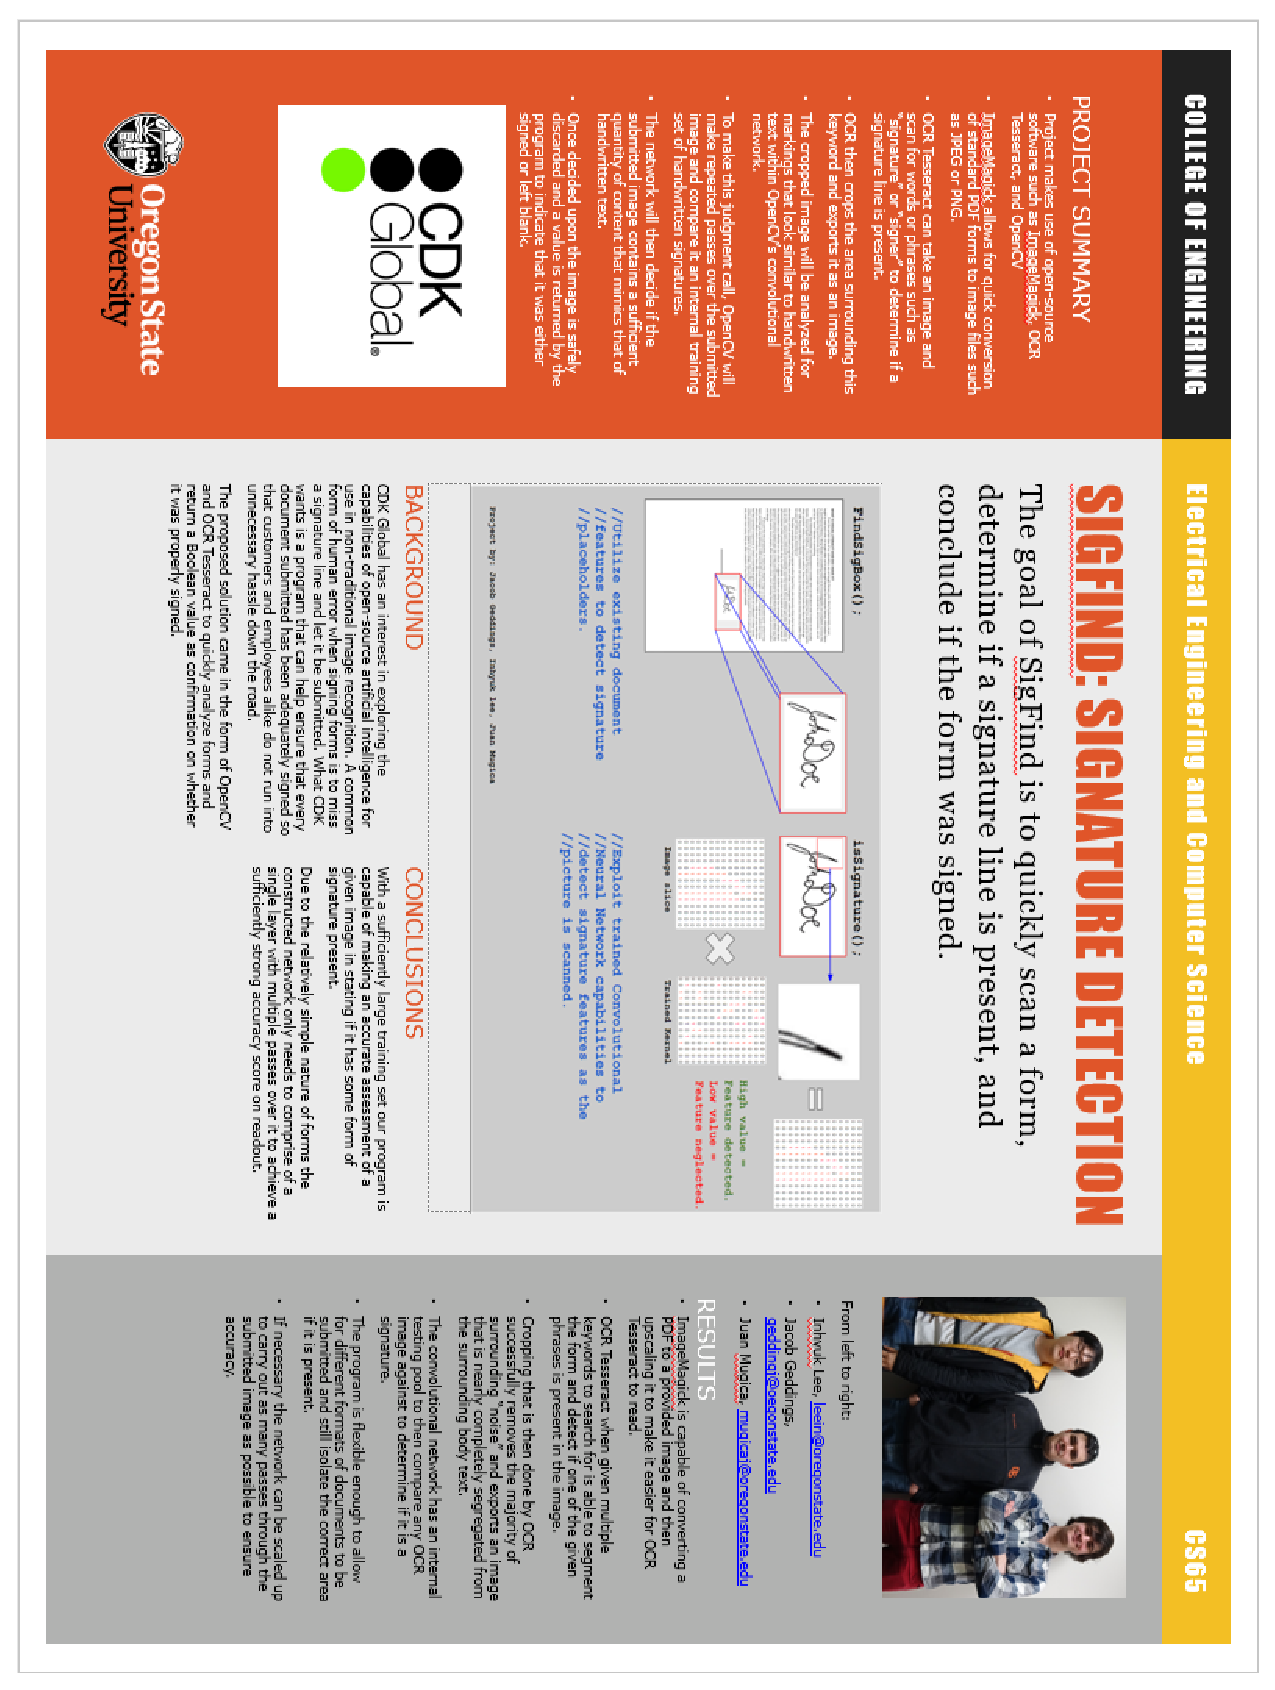
\includegraphics[width=\textwidth]{poster}
\end{figure}

\section{Project Documentation}
\subsection{How does your project work?}
Picture for a second a scenario that happens all too often in businesses all around the globe. In an obscure business department somewhere there sits an employee whose sole job is sifting through legal documents. When sifting through these, the main goal is to ensure that they have been processed correctly, which often comes down to whether they are signed or not. Usually legal documentation will be very long only containing a small subset of pertinent documents that are either signed or must be signed. The only solution nowadays is for someone to personally scroll through all of these documents in order to find out which ones should be looked at. But what if there was a program that could find signatures or lines that are supposed to be signed on any document no matter the format? This is what SigFind does and here’s how it does it. First it scans the document using OCR Tesseract which turns images of characters into characters readable by a computer. Once this is done it allows us to look for signature placehodlers such as “sign here” or “signature”. Once we have pinpointed where possible signatures could be found, we generate a box around signature lines or spaces. This signature is then passed into a Convolutional Neural Network, a neural network specifically designed to classify pictures. This specific neural network has been trained to understand many different signature patterns by being shown real human signatures hundreds of thousands of times. If the network deems that the box indeed contains a signature, it will highlight the area green, if it does not, it will highlight red. If any of the documents scanned has a signature line or a signature, it will be saved into a completely separate directory and renamed to include how many signatures are contained and how many unsigned lines there are. Now this absurdly mundane task is completely automated and our frustrated worker can find a better job. 

\subsection{Installation}
To setup ImageMagick, OpenCV, and Tesseract OCT, we need to set up Linux Subsystem on Windows.

All you need to do is installing ubuntu app on windows store.

This is the link that shows the instruction how to set up Linux subsystem.

https://docs.microsoft.com/en-us/windows/wsl/install-win10

\subsubsection{OpenCV (3.3.1 version) installation:}

Type the following steps on the command line.

sudo apt-get install build-essential

sudo apt-get install cmake git libgtk2.0-dev pkg-config libavcodec-dev libavformat-dev libswscale-dev

sudo apt-get install python-dev python-numpy libtbb2 libtbb-dev libjpeg-dev libpng-dev libtiff-dev libjasper-dev libdc1394-22-dev

cd ~/$<$my\_working \_directory$>$

Go to https://opencv.org/releases.html and download source code

cd ~/opencv

mkdir release

cd release

cmake -D CMAKE\_BUILD\_TYPE\$=RELEASE -D CMAKE\_INSTALL\_PREFIX\$=/usr/local ..

make -j8

sudo make install

For compiling convenience, do following steps.

After following the instruction, you just need to compile with `pkg-config opencv --cflags --libs` option in g++

sudo vim /etc/ld.so.conf.d/opencv.conf

	\# note: that is a lowercase 'L'

\# type this into the file

/usr/local/lib

\# exit out of file and enter:

sudo ldconfig

sudo vim /etc/bash.bashrc

\# in the newly opened file:

\# type this at the bottom of the file

PKG\_CONFIG\_PATH=\$PKG\_CONFIG\_PATH:/usr/local/lib/pkgconfig

export PKG\_CONFIG\_PATH

sudo apt-get install execstack

sudo /usr/sbin/execstack -c /usr/local/lib/libopencv\_*


\subsubsection{Leptonica and Tesseract OCR installation:}

Currently, newest version of tesseract OCR has compile error, so we need to install 3.0.5 version. 3.0.5 version is the most newest stable version.

Leptonica

\# remove tesseract binaries and languages

sudo apt-get remove tesseract-ocr*
 
\# remove leptonica

sudo apt-get remove libleptonica-dev
 
\# make sure other dependencies are removed too

sudo apt-get autoclean

sudo apt-get autoremove --purge
 
\# install required libraries

sudo apt-get install autoconf automake libtool

sudo apt-get install autoconf-archive

sudo apt-get install pkg-config

sudo apt-get install libpng12-dev

sudo apt-get install libjpeg8-dev

sudo apt-get install libtiff5-dev

sudo apt-get install zlib1g-dev

sudo apt-get install libicu-dev

sudo apt-get install libpango1.0-dev

sudo apt-get install libcairo2-dev

sudo apt-get install libtool



\# Install leptonica-1.75.2

Go to http://www.leptonica.org/download.html and download source file

cd leptonica

autoreconf -i 

./autobuild

./configure

sudo make

sudo make install

tesseract-OCR (3.0.5v)

Download source from this link: https://lucacerone.net/2017/install-tesseract-3-0-5-in-ubuntu-16-04/

Copy the source file from your windows to Linux subsystem.

cp /mnt/$<$drive$>$/User/your user name/location of the source file ~/location that you wants to install.

Note: you can access windows repositories from Linux subsystem from /mnt/

Unzip the file

cd tesseract

./autogen.sh

./configure --enable-debug

LDFLAGS="-l/usr/local/lib" CFLAGS="-i/usr/local/include" make

sudo make install

sudo make install -langs

sudo ldconfig

To extract text from image file, you need to install tessdata (trained set of data).

Download tessdata from this link: https://lucacerone.net/2017/install-tesseract-3-0-5-in-ubuntu-16-04/

This tessdata includes many languages, if you need only English, you can copy only English data to tessdata repository.

Copy the tessdata and copy it to the /usr/share/tesseract-ocr/tessdata or similar to this.

(if that does not work try /usr/local/share/tessdata)

^^ sudo cp 

\subsubsection{ImageMagick:}

sudo apt-get install ghostscript

sudo apt-get install libgs-dev

sudo apt-get install gs-esp

sudo apt-get --purge remove imagemagick

Get the source of ImageMagick, untar it, cd ImageMagick-xx

./configure --with-gslib=yes [and what else you need]

Confirm in the output near the bottom gslib yes yes and not gslib yes no

make

make install

\subsubsection{Graphical Applications:}

https://seanthegeek.net/234/graphical-linux-applications-bash-ubuntu-windows/

In order to run Linux GUI applications on Bash On Ubuntu on Windows, you must:
 
Install a X server for Windows

Configure bash to tell GUIs to use the local X server

Install VcXsrv

In order to run graphical Linux applications, you will need an X server.
 
VcXsrv is the only fully open source and up-do-date native X server for windows.
 
Download and run the latest installer

Run XLaunch

Press Next three times and press finish button.

A X icon will appear in your system tray.
 
Configure bash to use the local X server

In bash run:

echo "export DISPLAY=localhost:0.0" $>$$>$ ~/.bashrc

To have the configuration changes take effect, restart bash, or run:

. ~/.bashrc

Test a graphical application

Install x11-apps

sudo apt-get install x11-apps

Run xeyes

A new window will open, containing a pair of eyes that will follow your mouse movements.

\subsubsection{Compiling example:}

g++ sample.cpp -o sample `pkg-config opencv --cflags --libs` -llept -ltesseract

\subsection{How to run the program}
You just need to place all the pdf documents in form\_bin directory and type bash header\_bash on command line.

\section{Technical Resources}
\subsection{CONVOLUTIONAL NETWORK RESOURCES}
Below are the four most pertinent learning tools used for the creation of our network and understanding how it works. The first source breaks down the architecture associated with a convolutional network. The second and third sources are videos to help dissect the mathematical nature behind these networks. Lastly, the final source showcases how the layers of a network function and how the underlying math is applied to a given image when processing it.

“Convolutional Neural Network” ufldl.standford.edu. [Online]. Available: http://ufldl.stanford.edu/tutorial/supervised/ConvolutionalNeuralNetwork/. [Accessed Jan. 3, 2018].

S. Raval, “Convolutional Neural Networks – The Math of Intelligence (Week 4)” youtube.com, Jul. 12, 2017. [Online]. Available: https://www.youtube.com/watch?v=FTr3n7uBIuE. [Accessed Jan. 2, 2018].

L. Serrano, “A friendly introduction to Convolutional Neural Networks and Image Recognition” youtube.com, Mar 20, 2017. [Online]. Available: https://www.youtube.com/watch?v=2-Ol7ZB0MmU. Accessed [Jan. 3, 2018].

A. Deshpande, “A Beginner’s Guide To Understand Convolutional Neural Networks” github.io, Jul. 20, 2016. [Online]. Available: https://adeshpande3.github.io/adeshpande3.github.io/A-Beginner%27s-Guide-To-Understanding-Convolutional-Neural-Networks/. [Accessed Jan. 3, 2018].

\subsection{OCR TESSERACT}
Below are the three most helpful sources we discovered when trying to conceptualize how OCR Tesseract would work for us. The first source goes into detail on just what Optical Character Recognition is and how computers can be used for this end. The next source covers a basic tutorial on how to make OpenCV work with handwritten classifications of values. Lastly, we have an OCR Tesseract API library that works in conjunction with the OpenCV library. 

C. Woodford, “Optical character recognition (OCR)”, explainthatstuff.com, Jan. 2, 2018. [Online]. Available: https://www.explainthatstuff.com/how-ocr-works.html. [Accessed Feb. 20, 2018].

S. Mallick, “Handwritten Digits Classification : An OpenCV ( C++ / Python ) Tutorial” leanopencv.com, Jan. 30, 2017. [Online]. Available: https://www.learnopencv.com/handwritten-digits-classification-an-opencv-c-python-tutorial/. [Accessed Feb. 22, 2018].

“OCRTesseract Class Reference” opencv.org. [Online]. Available: https://docs.opencv.org/3.4.0/d7/ddc/classcv\_1\_1text\_1\_1OCRTesseract.html. [Accessed Feb. 18, 2018].

\section{Conclusions and Reflections}
\subsection{Jacob Geddings}
\subsubsection{What technical information did you learn?}
This project was entirely new to me in scope and subject matter. While I did have experience with the languages we decided to go with, that was where my experiences ended. As a result, some of the new technical information that I had to pick up on was how image processing AI operates. Learning about convolutional networks as well as the kernel, layering, and filtering within them was very different from anything I’ve had to study before. Beyond just the network itself the use of OCR Tesseract required new knowledge in page analysis as well as the function calls necessary to merge these two libraries together so that we could make use of their independent strengths.

\subsubsection{What non-technical information did you learn?}
As for non-technical knowledge there was a lot of research that went into understanding what makes all of the major open-sourced artificial intelligence good. When looking at our options I had to learn just what would make OpenCV our best choice when considering how best to interpret images. Another non-technical bit of information that I had to learn was using all of these new API libraries for ImageMagick, OCR Tesseract, and OpenCV. While they themselves would likely be considered technical the usage of them was anything but. Not only was the process of finding the documentation for these libraries a challenging experience but also deciding on what version we would use and on what platform.

\subsubsection{What have you learned about project work?}
Where a lot of my work went into was the general non-coding work associated with working with a client, teammates, and without the usual deadlines. In this environment I learned a great deal about the development cycle for creating projects such as these. In particular, the amount of paperwork that goes into them before even a single line of code is written down is incredible. What is amusing, or not so amusing, about this fact is that even though we spend months planning our project we almost immediately found small nuances we hadn’t accounted for or got wrong in our initial impressions of how this project would go despite the careful planning.

\subsubsection{What have you learned about project management?}
From a managing perspective this was a great opportunity for me to gain experience with leading a CS related team towards the completion of a project. The challenges associated with ensuring timelines are upkept and deadlines are being met was not something I really appreciated before this course. Assigning new meeting times, documenting what was said during meetings, and figuring out what the important takeaways of those meetings were proved to be a lot more demanding and enjoyable than I had initially figured them to be. One of the more stressful bits about this leadership position was the requirement to communicate with our client, as the lead communicator I had to get comfortable with talking to an individual as a ‘client’ as well as our grader.

\subsubsection{What have you learned about working in teams?}
As for the teamwork itself it wasn’t particularly new in nature. While my role within it was significantly different from previous courses the idea of working alongside other students is not. Some interesting developments we had included learning to cope with the schedule changes that’d occur every term when planning our meeting times. Another part was deciding on how to break up the work, without the usual graded assignment that has this sort of planning baked into it, we had to go about determining workload on our own. Lastly, handling when a group member becomes unresponsive to communication was something we learned to plan ahead for rather than allow it to seize up operations on the project.

\subsubsection{If you could do it all over, what would you do differently?}
If we could go back and do this entire project over there would be several changes I’d want to make. Firstly, when communicating with the client we failed to really gain metrics on the required component of the project and instead focused on the stretch goals for far too long. We also didn’t evenly divide the work that was associated per member moving into the Winter term, now knowing how much work the various components ultimately became it would have been more efficient to break those up from the start in a more even manner rather than having members hopping around on work. I’d also consider the use of a different language in the end, while we had clearly outlined why we wanted to go with C++, namely it’s performance capabilities, we would eventually realize that performance wasn’t vital and we are mostly just proving a concept. For concept proofing it would have been significantly easier to just develop in either Java or Python.


\subsection{Juan Mugica}
\subsubsection{What technical information did you learn?}
At the beginning of this project, I had basically no technical understanding of the tools and methods that we would implement for our solution. My specific part of the project was to implement a Convolutional Neural Network to understand and classify handwritten signatures, something which had fascinated me for a while, but of which I had no technical understanding. The first task that I had to tackle was to understand the inner workings of Convolutional Neural Networks, more specifically, what did the input look like, how was it addressed throughout the network, and what did the output look like. In a rather summed up manner, here’s what I learned.

A Convolutional Neural Network starts with a picture input, that is treated as a matrix. To any computing device, an image is a collection of red, green, and blue values, that is every pixel is assessed on the intensity of each of these colors, e.g. a blue pixel would have value of the form (0,0,255). These values range from 0-255 and when looked at as numbers, create a grid of values that can be treated as a matrix whose dimension is the width-1 and whose number of rows are the height. The next integral part of a convolutional network are the feature kernels or feature matrices. These matrices will eventually determine how close our input is to the desired classification, but more on that later. These feature kernels will always be much smaller than the picture matrix and are multiplied across this one. After being multiplied, its members are added up giving us a feature proximity value from the area in which they were multiplied. Once this feature matrix has been scanned throughout the picture, we end up with a smaller matrix consisting of the added-up elements of our previous scan. This is called a convolution.  The next layer is called a ReLu layer, which stands for rectified linear units. These layers are given a threshold minimum, which if a number is under, it will be rectified to 0. This is a strategy utilized to get the most out of matrix multiplication, ensuring that parts of the picture that are not relevant to our target classification hold the least level of importance possible. The next layer is a Max Pooling layer. This layer aims to decrease the load over the network by looking at square subsets of our matrix, and picking the highest value, once again these are the key values we will use to later classify. These steps are repeated as many times as one desires ending in an array of values passed on to a Fully Connected layer. A Fully Connected Layer takes on the conventional neural network architecture. It is a set of layers containing nodes which are fully connected to the next layer, that is every node is connected to every succeeding node. These nodes apply an activation function, meaning they either carry on input, or do not. Fully Connected layers can have binary or classificatory outputs depending on the number of things we would like our network to understand. 

To train these networks an image input is passed on and ran through the network. The parameters within these (the feature kernels, as well the weights within the fully connected network), are at first fully randomized. The first output will be pretty random except for it gives us a cost, which is the difference between an expected output and our actual output. In essence, all Neural Networks are minimizing a cost functions, whose parameters are the aforementioned kernels and fully connected network weights. After a pass, an optimization is performed which tells the network whether the route taken by the input was erroneous or correct. This optimization modifies the weights within the network as well as the kernel matrix values, all dependent on which triggered the response, or in the features kernels where the response was triggered. Eventually, our feature kernels will start to look like parts of our picture, which when multiplied against our input will yield high values. 

Moreover I had to learn how to implement and work with OpenCV, a computer vision library which enables pixel manipulation, image representation, saving, etc. Beginning to work with it was a daunting task given a widely ranging number of implementations, languages, and documentations. Towards the end of the project, it proved to be an extremely powerful tool for any computer vision program imaginable. 

\subsubsection{What non-technical information did you learn?}
The most important thing that I learned throughout this course is the value of putting in consistent amounts of work, over long periods of time. As a bit of a procrastinator, I was rather used to seeing the fruit of my work come together in 9-12 hours but seeing the sheer amount of parts created for this project, all working together, to provide a working solution to our problem was a feat that made me realize I had been doing it wrong all along. Not that I ever thought it was the most efficient way, but I digress. 

\subsubsection{What have you learned about project work?}
Communication is by far the most important element of any project. When a task takes putting many parts together, it is crucial to efficiently delegate tasks and efficiently communicate progress. It is not always easy to tell what will take a long time and what will not, which is why it is essential that progress be communicated, and resources relocated if necessary. Moreover, learning to take and give constructive criticism. When a specific goal is at hand, one should seek to put all personal problems away and communicate in the same manner. Being condescending, rude, mean, does not foster progress, and neither does being defensive, elusive, or evasive. 

\subsubsection{What have you learned about project management?}
As contrary as it may seem, I learned that project management should be handled by the least number of people possible, albeit competent. There should be a trusted leader who is able to recognize and hand out tasks efficiently. This process can get extremely tricky if everyone is trying to call the shots and nobody trusts each other. 

\subsubsection{What have you learned about working in teams?}
Once again, the most important part is communication. It’s ok to be late, it’s ok if certain parts do not work correctly, but it is not okay to not let your group members know. Nobody wants to seem like they are not doing their job, and one should always be doing their job. But life can get difficult, schedules can become unreasonable and all of these things should be reported and understood. At the end of the day, you are a team, and whether it be for the best or the worst, you must carry your team when they need it, and be ready to be carried when goals seem unachievable. 

\subsubsection{If you could do it all over, what would you do differently?}
I’m not gonna lie, I have appreciated essentially every single part of this course, whether it be bad or good, I think there were lessons to be learned in the bad and feel very proud of the good. Being very objective here, I would say that the most important thing is to not relax just because there is a lot of time, and not because you won’t reach the deadline, but rather because your project could have been that much better. 

\subsection{Inhyuk Lee}
\subsubsection{What technical information did you learn?}
I have learned many things from this project. Since none of our group member had back ground knowledge on image processing or artificial intelligence, we had to start from learning it. I have learned how optical character recognition works and how convolutional neural network works. In coding wise, now I know how to use Tesseract OCR API to convert image into machine readable text and how to use basic functions of OpenCV to perform image processing. 

\subsubsection{What non-technical information did you learn?}
None of our group members had back ground knowledge, and we had no advisor to teach us the information. We had to research everything from the scratch. It was very difficult; however, it was valuable experience. I learned how to do get the information that I want and learned how to learn new things. 

\subsubsection{What have you learned about project work?}
From this project, I learned two things about project work. I learned how to communicate in group and leaned how to divide work equally to work efficiently. I felt that these skills were very important through out the year, and I believe our group did very well on communicating with each other’s and dividing works fairly. For communicating, we had three weekly meeting. If one of the group member miss the meeting, other group members let him know what they did during the meeting or reschedule the meeting time. For work division, we splitted the work into similar portion. Usually we worked individually, and we sum up the work when all the work is done.

\subsubsection{What have you learned about project management?}
For me, I learned how time management is critical and difficult in group project. Since all of our group member had different schedule, it was difficult to schedule the meeting time and divide the work at first, so we ask each group members schedule when we have assignments due or need meeting. If we could not have meeting, we rescheduled the meeting time or opened up the Webex meeting. Also, if one of the group member is too busy to work on project, other group member covered up his work.

\subsubsection{What have you learned about working in teams?}
As I mentioned above, I learned how to communicate with other group members, divide work fairly, and set schedule that satisfy all the group members. I felt these skills are very important to work successfully as a group, and we did great on it. We had three meeting every week, and on the meeting, we shared each group member’s progress. We also split the work as fair as possible and set schedule that all group member can be satisfied.

\subsubsection{If you could do it all over, what would you do differently?}
If I can do it all over, I would like to change the way how we split our work. Our group split the work into three parts which are image conversion part, signature location part, and signature detection part. It makes sense, and it worked well. However, since we split work in this way, all group members do not know details on other member’s part. We do roughly know how it works since we shared our progress on every week, but we do not know enough to help each other. Also, since image converting part was simple compare to other parts, Jacob mostly worked on non-coding stuffs. If we had divided the work differently, he would have learned more on artificial intelligence and image processing. In my case, I know how our convolution neural network works, but do not know how to hard code it.

\section{Appendix 1: Essential Code Listings}
\begin{figure}
  \caption{forwardPass code 1}
  \centering
  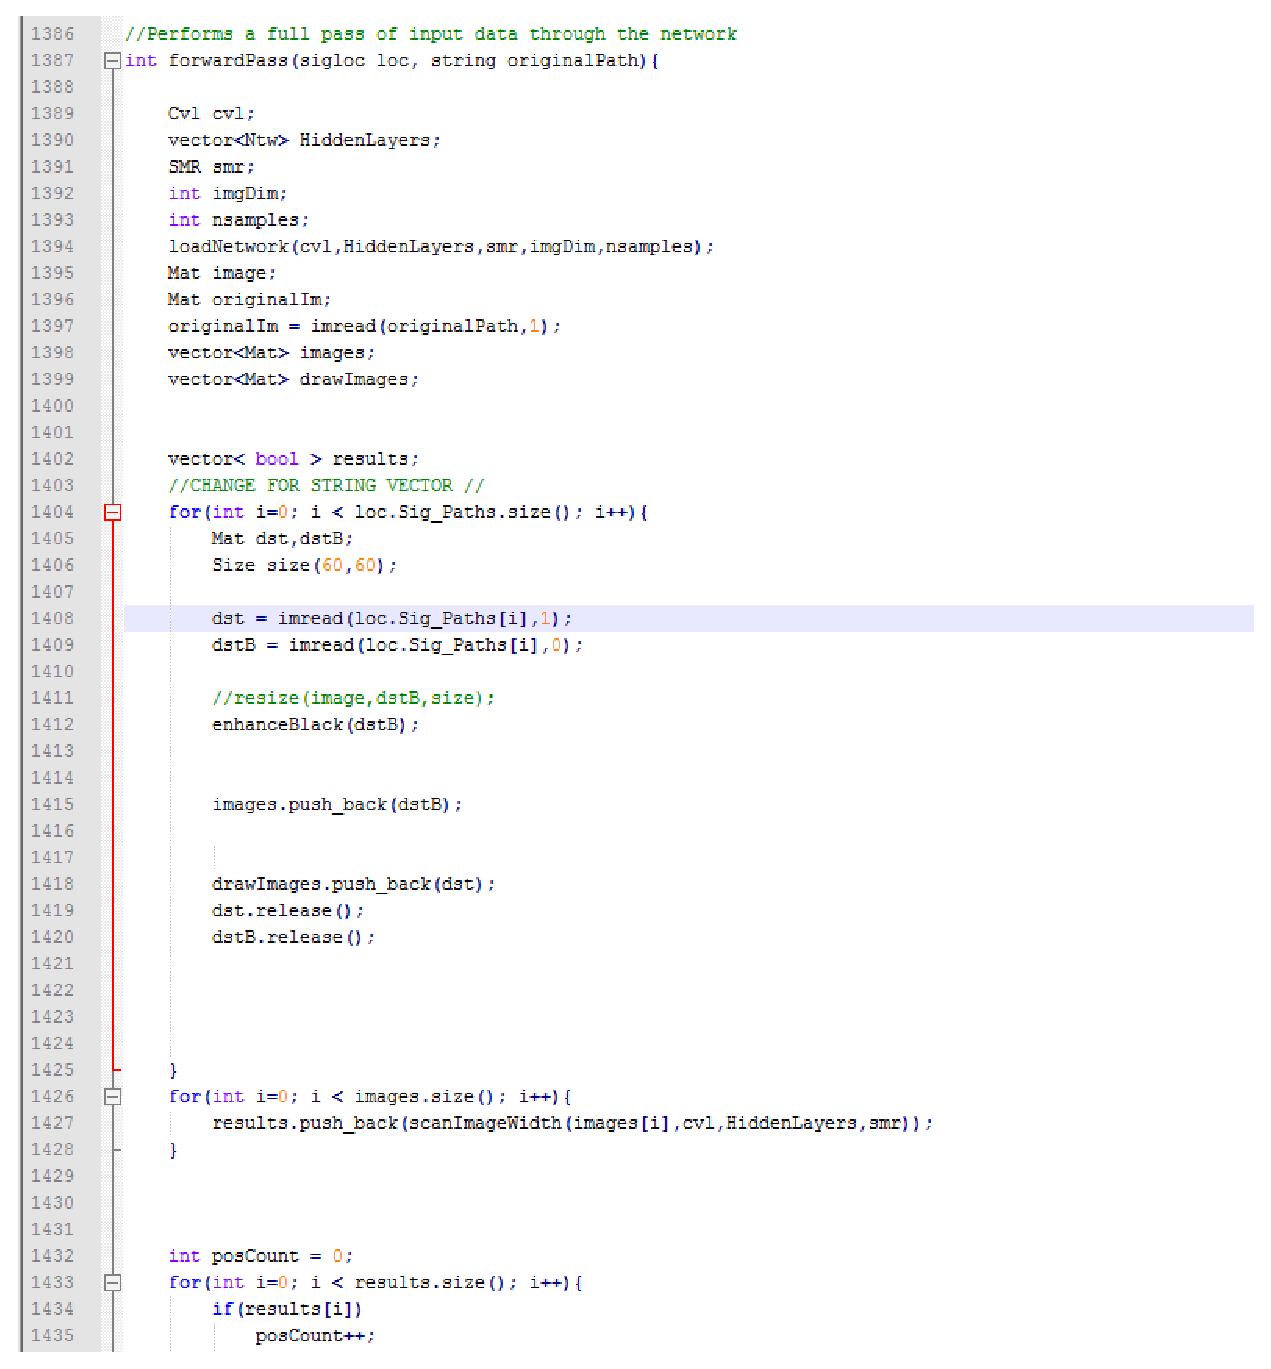
\includegraphics[width=\textwidth]{forwardPass1}
\end{figure}
\begin{figure}
  \caption{forwardPass code 2}
  \centering
  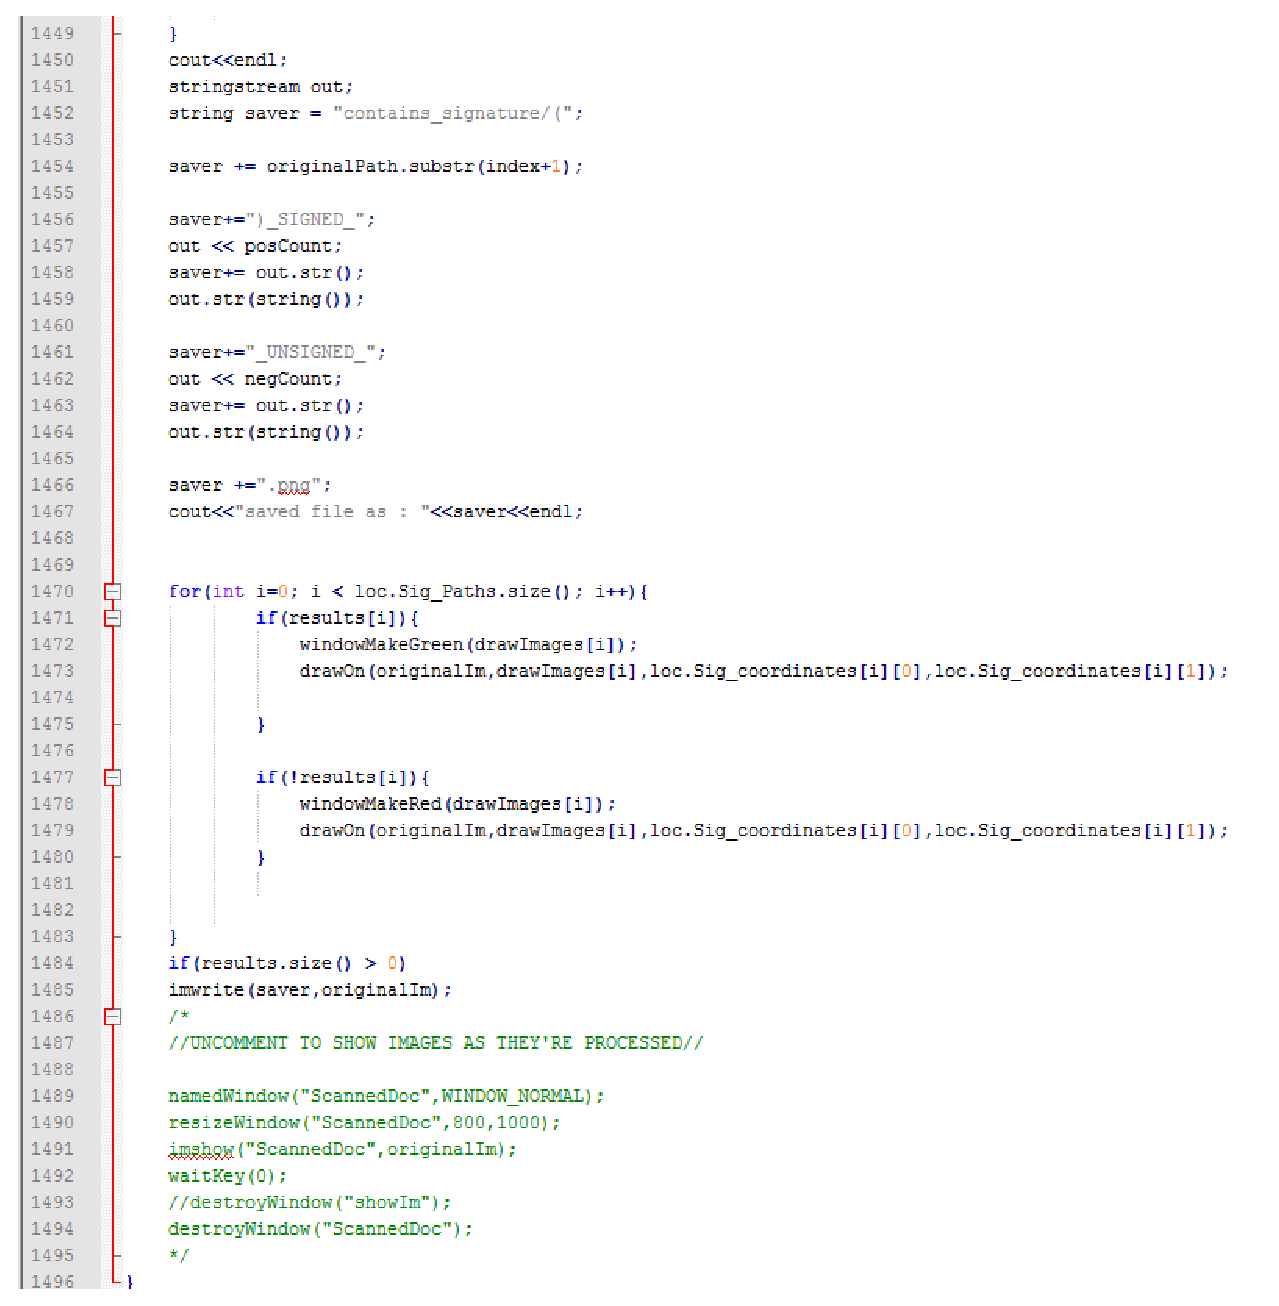
\includegraphics[width=\textwidth]{forwardPass2}
\end{figure}
\begin{figure}
  \caption{loadNetwork code 1}
  \centering
  \includegraphics[width=\textwidth]{loadNetwork1}
\end{figure}
\begin{figure}
  \caption{loadNetwork code 2}
  \centering
  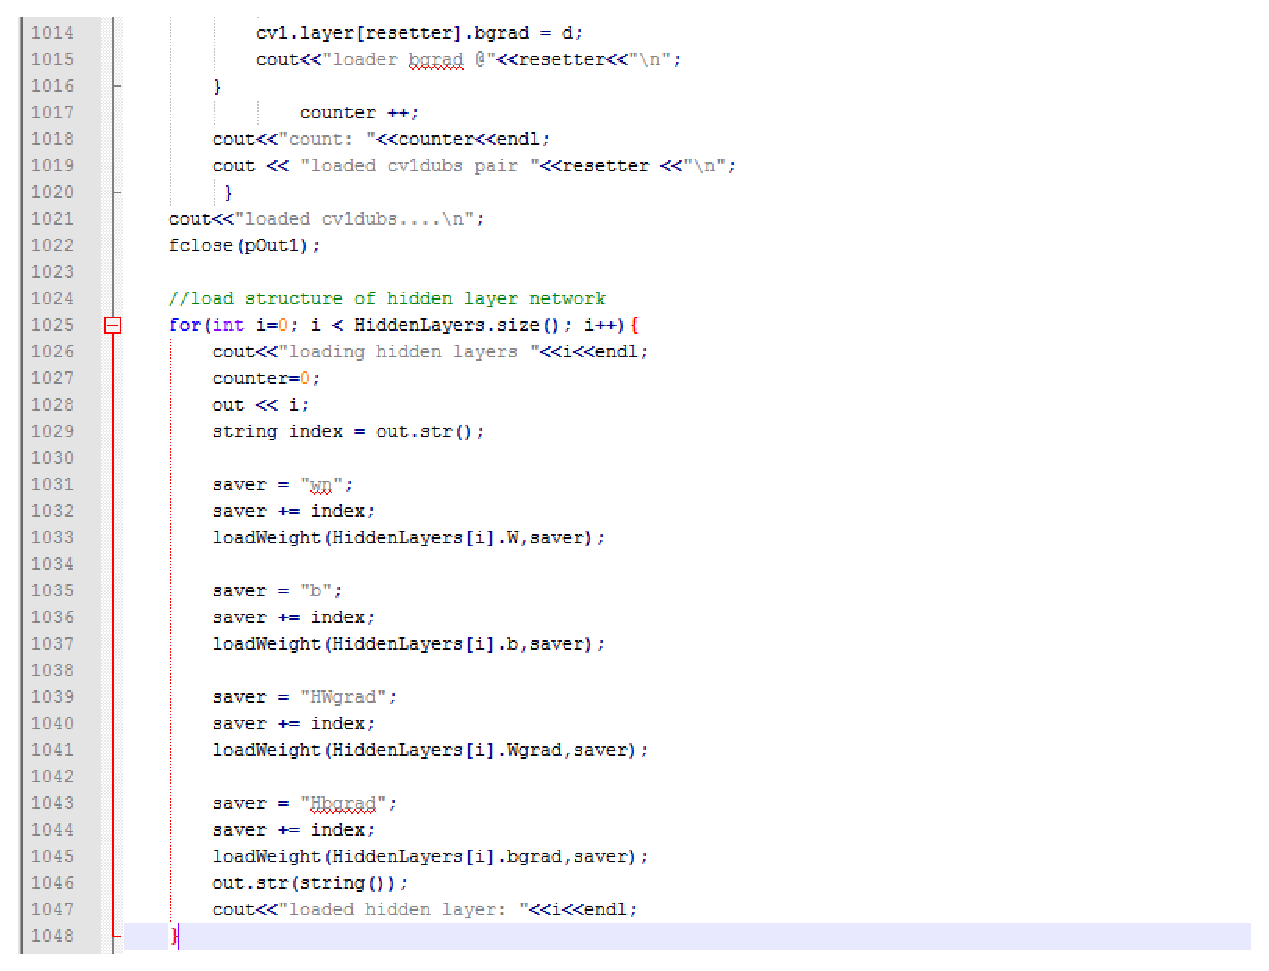
\includegraphics[width=\textwidth]{loadNetwork2}
\end{figure}
\begin{figure}
  \caption{loadNetwork code 3}
  \centering
  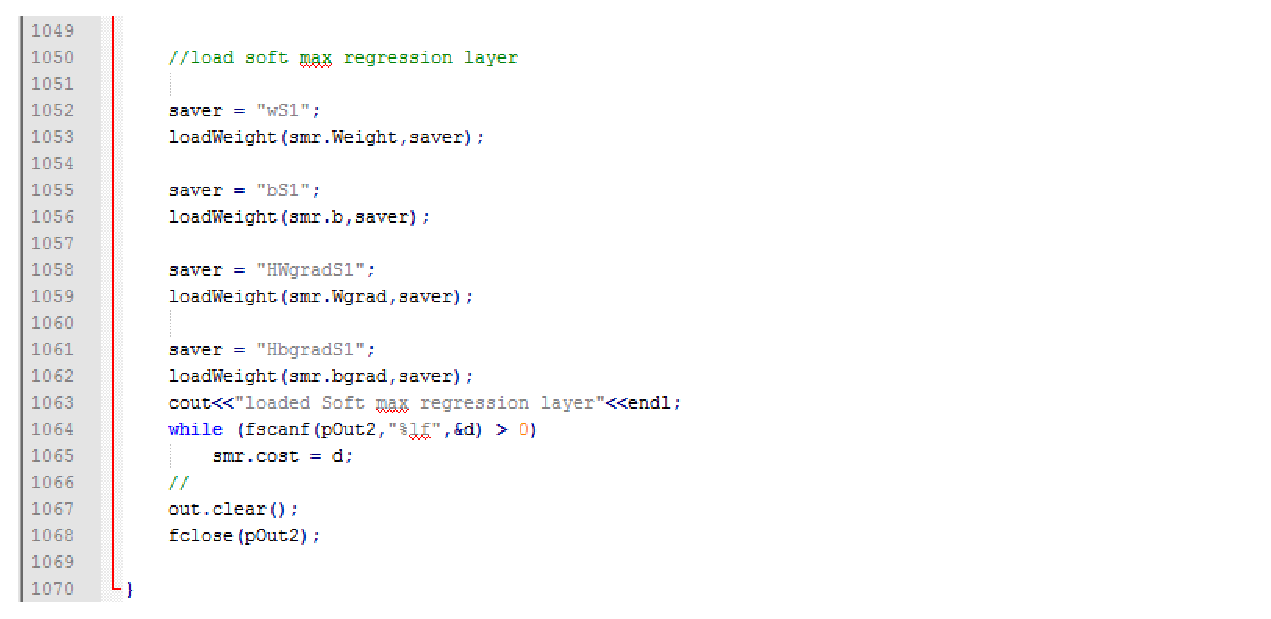
\includegraphics[width=\textwidth]{loadNetwork3}
\end{figure}
\begin{figure}
  \caption{resultProdict code 1}
  \centering
  \includegraphics[width=\textwidth]{resultProdict}
\end{figure}
\begin{figure}
  \caption{resultProdict code 2}
  \centering
  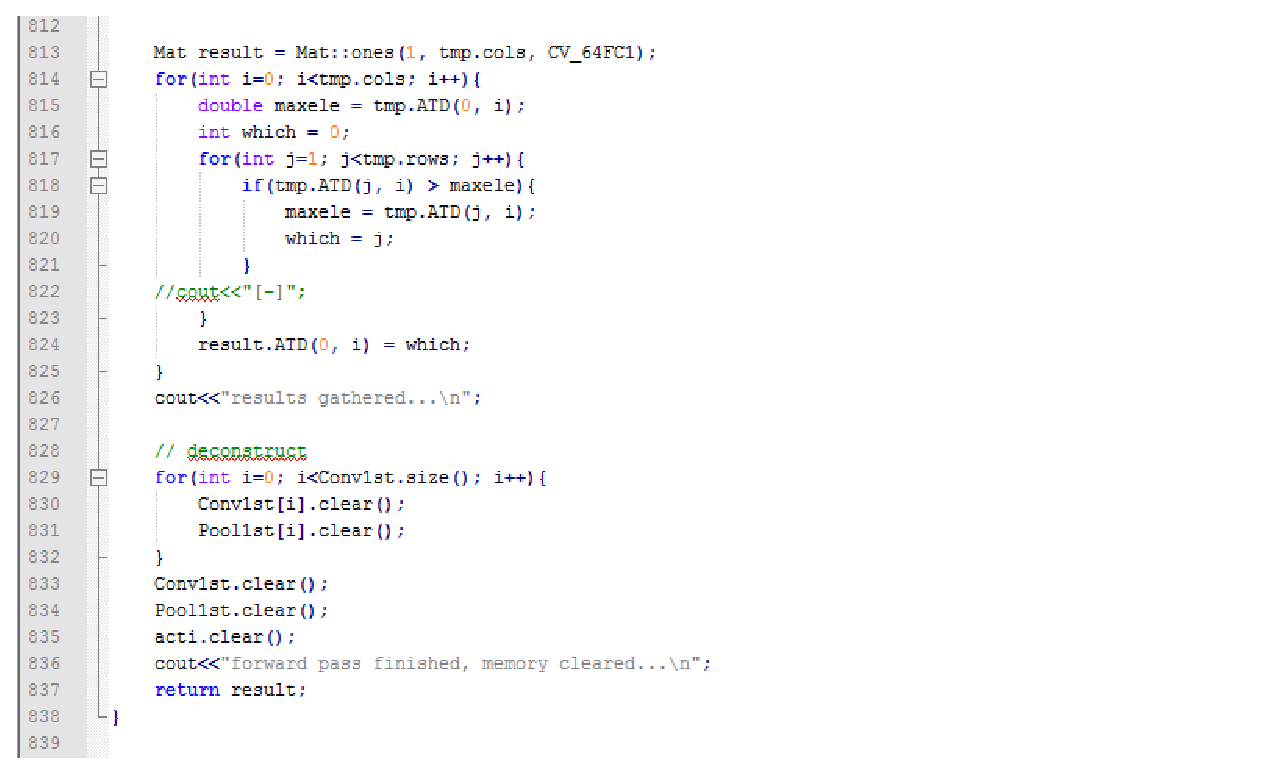
\includegraphics[width=\textwidth]{resultProdict2}
\end{figure}
\begin{figure}
  \caption{saveNetwork code 1}
  \centering
  \includegraphics[width=\textwidth]{saveNetwork1}
\end{figure}
\begin{figure}
  \caption{saveNetwork code 2}
  \centering
  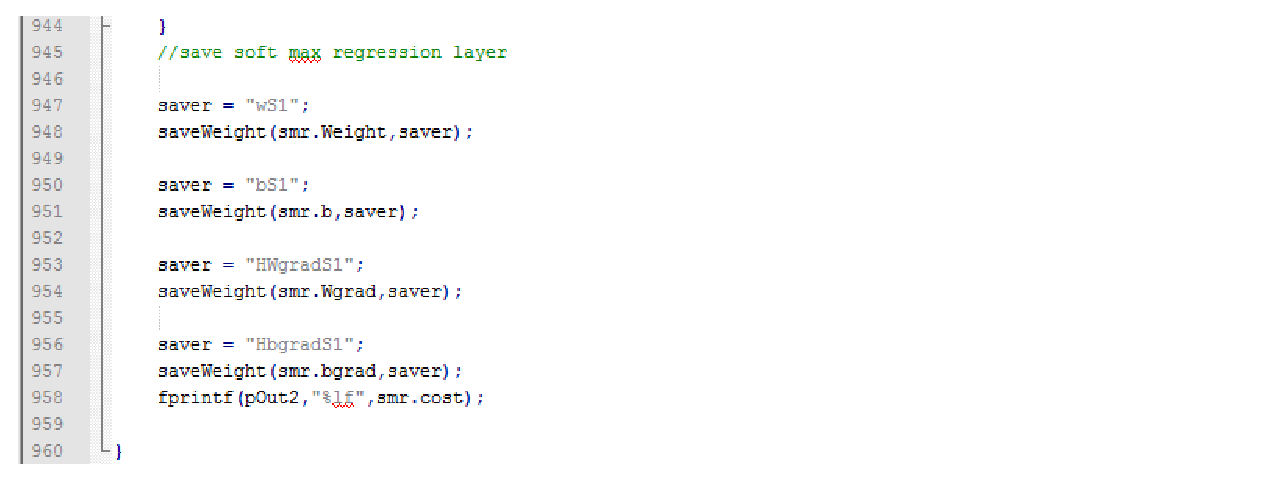
\includegraphics[width=\textwidth]{saveNetwork2}
\end{figure}
\begin{figure}
  \caption{saveWeight\&LoadWeight code}
  \centering
  \includegraphics[width=\textwidth]{saveWeight&LoadWeight}
\end{figure}
\begin{figure}
  \caption{scanImage code 1}
  \centering
  \includegraphics[width=\textwidth]{scanImage1}
\end{figure}
\begin{figure}
  \caption{scanImage code 2}
  \centering
  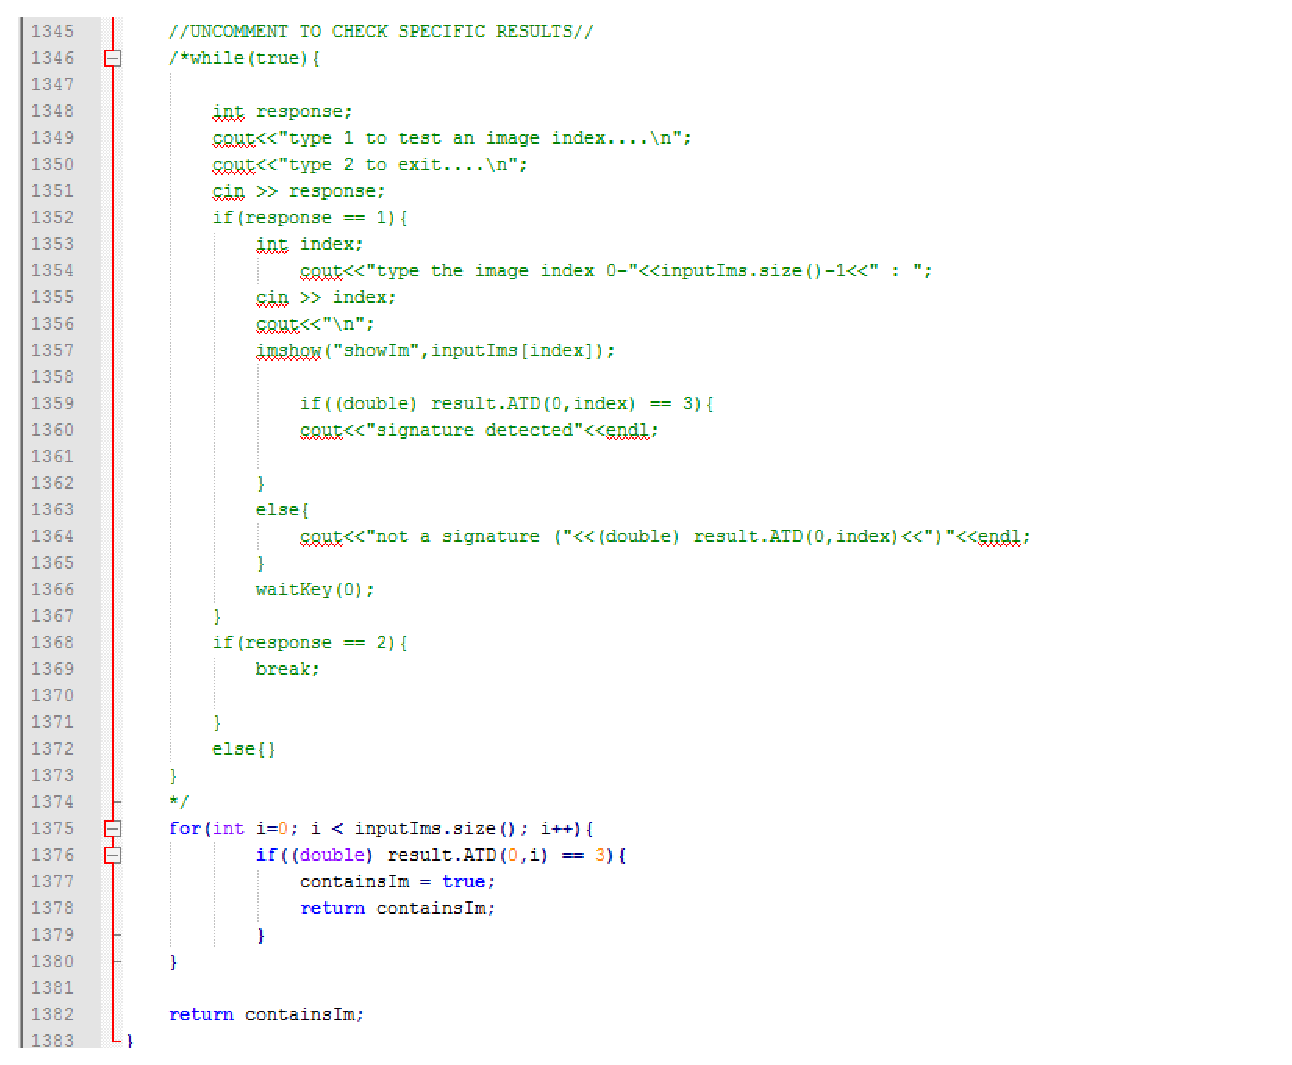
\includegraphics[width=\textwidth]{scanImage2}
\end{figure}
\begin{figure}
  \caption{trainNetwork code }
  \centering
  \includegraphics[width=\textwidth]{trainNetwork}
\end{figure}

\end{document}